\documentclass[aps, prd, twocolumn, superscriptaddress, floatfix, showpacs, nofootinbib, longbibliography]{revtex4-1}

% Fixes Adbobe error (131)
\pdfminorversion=4

% Ams math
\usepackage{amsmath}
\usepackage{amssymb}

% Packages for setting figures
\usepackage[]{graphicx}
\usepackage{subfig}

% Colors
\usepackage{color}

% Bibliography
\usepackage{natbib}

\usepackage{placeins}

\usepackage{multirow}

\usepackage{hhline}

% get hyperlinks
%\usepackage{hyperref}

% Tables
\newcommand{\specialcell}[2][c]{%
  \begin{tabular}[#1]{@{}c@{}}#2\end{tabular}}

\newcommand{\fdot}{\dot{f}}
\newcommand{\F}{{\mathcal{F}}}
\newcommand{\twoFhat}{\widehat{2\F}}
\newcommand{\twoFtilde}{\widetilde{2\F}}
\newcommand{\A}{\boldsymbol{\mathcal{A}}}
\newcommand{\blambda}{\boldsymbol{\mathbf{\lambda}}}
\newcommand{\blambdaSignal}{\boldsymbol{\mathbf{\lambda}}^{\rm s}}
\newcommand{\tglitch}{t_{\rm glitch}}
\newcommand{\tstart}{t_{\rm start}}
\newcommand{\tend}{t_{\rm end}}
\newcommand{\Nglitches}{N_{\rm g}}
\newcommand{\Tspan}{T}
\newcommand{\Tcoh}{T_{\rm coh}}
\newcommand{\tref}{t_{\rm ref}}
\newcommand{\Nseg}{N_{\rm seg}}
\newcommand{\Nsteps}{N_{\rm steps}}
\newcommand{\Ntemps}{N_{\rm temps}}
\newcommand{\Nstages}{N_{\rm stages}}
\newcommand{\Nspindown}{N_{\rm spindowns}}
\renewcommand{\H}{\mathcal{H}}
\newcommand{\Hs}{\H_{\rm s}}
\newcommand{\Hn}{\H_{\rm n}}
\newcommand{\ho}{h_0}
\newcommand{\homax}{\ho^{\rm max}}
\newcommand{\Bsn}{B_{\rm S/N}}
\newcommand{\AmplitudePrior}{\Pi_\mathcal{A}}
\newcommand{\mutilde}{\tilde{\mu}}
\newcommand{\Sn}{S_{\rm n}}
\newcommand{\V}{\mathcal{V}}
\newcommand{\Vsky}{\V_{\rm Sky}}
\newcommand{\Vpe}{\V_{\rm PE}}
\newcommand{\smax}{s_{\textrm{max}}}
\newcommand{\fmax}{f_{\textrm{max}}}


\def\DirectedMCNoiseOnlyMaximum{52.4}
\def\DirectedMCNoiseN{10000}
\def\AllSkyMCNoiseOnlyMaximum{59.8}
\def\AllSkyMCNoiseN{10000}


% For editing purposes: remove before submition
\usepackage[normalem]{ulem}	%% only added for 'strikeout' \sout
\usepackage[usenames,dvipsnames]{xcolor}

\newcommand{\dcc}{LIGO-{\color{red}}}

%% ---------- editing/commenting macros: make sure all a cleared at the end! ----------
\newcommand{\mygreen}{\color{green!50!black}}
\newcommand{\addtext}[1]{\textcolor{green!50!black}{#1}}
\newcommand{\meta}[1]{\addtext{#1}}
\newcommand{\CHECK}[1]{\textcolor{red}{#1}}
\newcommand{\strike}[1]{\textcolor{red}{\sout{#1}}}
\newcommand{\comment}[1]{\textcolor{red}{[#1]}}
\newcommand{\replace}[2]{\strike{#1}\addtext{$\rightarrow$ #2}}
%% ---------- end: editing/commenting macros ----------------------------------------

\begin{document}

\title{MCMC follow-up methods for continuous gravitational wave candidates}

    \author{G. Ashton}
    \email[E-mail: ]{gregory.ashton@ligo.org}
    \affiliation{Max Planck Institut f{\"u}r Gravitationsphysik
                 (Albert Einstein Institut) and Leibniz Universit\"at Hannover,
                 30161 Hannover, Germany}
    \author{R. Prix}
    \affiliation{Max Planck Institut f{\"u}r Gravitationsphysik
                 (Albert Einstein Institut) and Leibniz Universit\"at Hannover,
                 30161 Hannover, Germany}

\date{\today}

\begin{abstract}

We detail methods to follow-up potential CW signals (as identified by
wide-parameter space semi-coherent searches) leveraging MCMC optimisation of
the $\mathcal{F}$-statistic. Such a framework provides a unique advantage when
used during the `zoom' (in which the coherence time is increased aiming to
localise the fully-coherent candidate) in that several candidates can be
effeciently followed up simultaneously. We describe an automated method to
define the number of zoom stages and verify such methods work in a Monte-Carlo
study. More, MCMC optimisation naturally produces parameter estimation for the
final fully-coherent candidate. Finally, we show that with minor modifications
the follow-up may allow for the CW waveform to be transient or undergo
glitches; this may allow the discovery of signals which would otherwise go
underdetected.

\end{abstract}

\pacs{04.80.Nn, 97.60.Jd, 04.30.Db}
\input{git_tag.tex}
\date{\commitDATE; \commitIDshort-\commitSTATUS, \dcc}

\maketitle


\section{Introduction}

A possible target for the advanced gravitational wave detector network of LIGO
and Virgo are long-lived periodic sources called continuous waves (CWs).
Rapidly rotating nonaxisymmetric neutron stars are potentially capable of
producing detectable CWs which last much longer than typical observation spans.
There exists three well known sources of the nonaxisymmetry: `mountains',
precession, and r-mode oscillations; each of which make a prediction for the
scaling between $\nu$, the NS spin frequency and $f$, the gravitational wave
frequency. In any case, observing neutron stars through their gravitational
wave emission would provide a unique astrophysical insight and has hence
motivated numerous searches.

As shown by \citet{jks1998}, the gravitational wave signal from a
nonaxisymmetric source produces a strain in the detector $h(t, \A, \blambda)$;
where $\A{=}\{h_0, \cos\iota, \psi, \phi_0\}$ is a vector of the four
\emph{amplitude-parameters} (expressed in `physical coordinates') and
$\blambda$ is a vector of the \emph{Doppler-parameters} consisting of the
sky-location, frequency $f$, and any spindown terms required by the search.

CW searches typically use a fully-coherent matched-filtering methods whereby a
template (the signal model at some specific set of parameters) is convolved
against the data resulting in a detection statistic. Since the signal
parameters are unknown, it is usual to perform this matched filtering over a
grid of points.  Three search categories can be identified: \emph{targeted}
searches for a signal from a known electromagnetic pulsar where the Doppler
parameters are considered `known'; \emph{directed} searches in which the
location is known, but not the frequency and spin-down (i.e.  searching for the
neutron star in a supernova remnant which does not have a known pulsar); and
\emph{all-sky} searches where none of the parameters are considered known.
Searching over more parameters amounts to an increase in the dimension of the
search space. Since the density of grid points required to resolve a signal
scales inversely with total coherence time $\Tcoh$ (the span of data used in
a fully-coherent matched filter), wide-parameter searches (such as the all-sky)
with many search dimensions over long durations of data are computationally
demanding.

At a fixed computing cost, it has been shown (see for example \citep{brady1998,
prix2012}) that a semi-coherent search is more sensitive for unknown signals
than a fully-coherent search. While the exact details of how the search works
depends on the implementation, semi-coherent search work by splitting the total
observation span $\Tspan$ into $\Nseg$ segments (each lasting for $\Tcoh$) and
in each segment computes the fully-coherent detection statistic; the
semi-coherent detection statistic is then computed by some combination of all
segments summed at the same point in parameter space. Fundamentally, this gain
in sensitivity is because the width of a peak in the detection statistic due to
a signal is inversely proportional to the coherence time: shorter coherence times
make the peak wider and hence the a lower density of templates. This idea was
first proposed by \citet{brady2000} along with the first implementation, the
`Stack-slide' search. Since then, several modifications such as the
`Hough-transform' \citep{krishnan2004, astone2014}, and the `Powerflux' method
(first described in \citet{allyskyS42008}) have been proposed, implemented and
applied to gravitational wave searches.

Wide parameter space searches produce a list of candidates with an associated
detection statistic which passes some threshold. In order to verify these
candidates, they are subjected to a \emph{followed-up}: a process of increasing
the coherence time, eventually aiming to calculate a fully-coherent detection
statistic over the maximal span of data. In essence, the semi-coherent search
is powerful as it spreads the significance of a candidate over a wider area of
parameter space, so a follow-up attempts to reverse this process and recover
the maximum significance and tightly constrain the candidate parameters. The
original hierarchical follow-up of \citet{brady2000} proposed a two-stage method
(an initial semi-coherent  stage followed directly by a fully-coherent search.
However, it was shown in a numerical study by \citet{cutler2005} that allowing
an arbitrary number of semi-coherent stages before the final fully-coherent
stage can significantly improve the efficiency: ultimately they concluded that
three semi-coherent stages provide the best trade-off between sensitivity and
computational cost.

The first implementation of a two-stage follow-up was given by
\citet{shaltev2013} and used the Mesh Adaptive Direct Search algorithm for
optimisation. At the time of publication, this method was limited to two stages
and could not handle binary parameters \comment{(I think these limitations have
now been removed, but I can't find a publication)}, however these are practical
limitations which can \comment{(have?)} be overcome.
\comment{Add something on multiple modes?}

In this paper, we propose an alternative hierarchical follow-up procedure using
Markov-Chain Monte-Carlo (MCMC) as the optimisation tool. In terms of the
semi-coherent to follow-up procedure, an MCMC tool is advantages due to it's
ability to trace the evolution multiple modes simultaneously through the
follow-up procedure and allow the optimisation to decide between them without
arbitrary cuts. In addition, MCMC methods also provide two further
advantages: they can calculate directly calculate Bayes factors, the significance
of a candidate and because they are `grid-less' one can arbitrarily vary the
waveform model without requiring an understanding of the underlying topology.
We will exploit this latter property to propose an additional step in the
follow-up procedure which allows for the CW signal to be either a transient-CW
(a periodic signal lasting $\mathcal{O}(\textrm{hours-weeks})$) or to undergo
glitches (as seen in pulsars).

We begin in Section~\ref{sec_hypothesis_testing} with a review of search
methods from a Bayesian perspective. Then in
Section~\ref{sec_MCMC_and_the_F_statistic} we introduce the MCMC optimisation
procedure and give details of our particular implementation. In
Section~\ref{sec_follow_up} we will illustrate applications of the method and
provide a prescription for choosing the setup. In Sections~\ref{sec_transients}
and \ref{sec_glitches} we demonstrate how searches can be performed for either
transient or glitches CWs before we finally conclude in
Section~\ref{sec_conclusion}.

\section{Hypothesis testing}
\label{sec_hypothesis_testing}

\subsection{Bayes factors}
Given some data $x$ and a set of background assumptions $I$, we formulate
two hypotheses: $\Hn$, the data contains solely Gaussian noise and $\Hs$, the
data contains an additive mixture of noise and a signal $h(t; \A, \blambda)$.
In order to make a quantitative comparison, we use Bayes theorem in the usual
way to write the odds as
\begin{equation}
O_{\rm S/N} \equiv \frac{P(\Hs| x, I)}{P(\Hn| x, I)} =
\Bsn(x| I) \frac{P(\Hs| I)}{P(\Hn | I)},
\end{equation}
where the second factor is the prior odds while the first factor is the
\emph{Bayes factor}:
\begin{equation}
\Bsn(x| I) = \frac{P(x| \Hs, I)}{P(x| \Hn, I)}.
\end{equation}
Typically, we set the prior odds to unity such that it is the Bayes factor
which determines our confidence in the signal hypothesis. In this work we will
therefore discuss the Bayes factor with the implied assumption this is
equivalent to the odds, unless we have a good reason to change the prior odds.

We can rewrite the Bayes factor in terms of the two sets of signal parameters
as
\begin{equation}
\Bsn(x| I) = \frac{P(x, \A, \blambda|\Hs, I)}
{P(\A| \Hs, I)P(\blambda| \Hs, I)P(x| \Hn, I)}.
\end{equation}
Marginalising over the two sets of parameters we find that
\begin{equation}
\Bsn(x| I)= \iint
\mathcal{L}(x; \A, \blambda)
P(\A| \Hs, I)P(\blambda| \Hs, I)
d\blambda d\A
\label{eqn_full_bayes}
\end{equation}
where
\begin{equation}
\mathcal{L}(x; \A, \blambda) \equiv \frac{P(x |\A, \blambda, \Hs, I)}{P(x| \Hn, I)},
\label{eqn_likelihood}
\end{equation}
is the \emph{likelihood-ratio}.

At this point, we can appreciate the problems of searching for unknown signals:
one has four amplitude parameters and several Doppler parameters (three plus
the number of spin-down and binary parameters) over which this integral must be
performed. If a single signal exists in the data, this corresponds to a single
peak in the likelihood-ratio, but at an unknown location. Therefore, one must
must first search for peaks (candidates), and then subsequently analyse their
significance. If one has prior knowledge this can be used; for example in
targeted searches for gravitational waves from known pulsars emitting CWs from
a mountain the Doppler parameters are considered known collapsing their
integral to a single evaluation.

\subsection{The $\F$-statistic}

For directed and all-sky searches, a common method introduced by
\citet{jks1998} to reduce the parameter space is the maximum-likelihood
approach. In this approach (often referred to as `frequentist'), one starts by
defining the likelihood-ratio, Equation~\eqref{eqn_likelihood}, which in this
context is a \emph{matched-filtering} amplitude. Then, analytically maximising
this likelihood-ratio with respect to the four amplitude parameters results
(c.f.~\citet{prix2009}) in a maximised log-likelihood given by $\F(x|
\blambda)$: the so-called $\F$-statistic. Picking a particular set of Doppler
parameters $\blambda$ (the template) one can then compute a detection statistic
(typically $2\F$ is used) which can be used to quantify the significance of the
template. Usually this is done by calculating a corresponding false alarm rate,
the probability of seeing such a detection statistic in Gaussian noise.

Calculations of the significance are possible due to the properties of the
detection statistic: in Gaussian noise, it can be shown \citep{jks1998,
cutlershutz2005} that $\widetilde{2\F}$ follows a chi-squared distribution with
4 degrees of freedom. In the presence of a signal, $\widetilde{2\F}$ is
still chi-squared with 4 degrees of freedom, but has a non-centrality parameter
$\tilde{\rho}^{2}$ such that its expectation value is
\begin{equation}
\textrm{E}[\widetilde{2\F}(x; \blambda)] = 4 + \tilde{\rho}(x; \blambda)^2.
\label{eqn_twoF_expectation}
\end{equation}
The non-centrality parameter in this context is the SNR of the matched-filter
given by
\begin{equation}
\rho^{2} = (h | h) \propto \frac{h_0^2}{\Sn}\Tcoh \mathcal{N}
\end{equation}
where $(h|h)$ is the inner product of the signal with itself (see for example
\citet{prix2009}), $\Sn$ is a (frequency-dependent) measure of the noise in
the detector and $\mathcal{N}$ is the number of detectors.


\subsection{Using the $\F$-statistic to compute a Bayes factor} At first, it
appears that the $\F$-statistic is independent of the Bayesian framework since
it was first derived directly from the likelihood. However, it was shown by
\citet{prix2009} that if we marginalise over the four amplitude parameters of
Equation~\eqref{eqn_full_bayes}, choosing a prior $\Pic$ such that
\begin{equation}
P(\A| \Hs, \Pic, I) \equiv \left\{
\begin{array}{ll}
C & \textrm{ for } \ho < \homax \\
0 & \textrm{ otherwise}
\end{array}
\right..
\end{equation}
then the integral, when $\homax \gg 1$, is a Gaussian integral and can be
computed analytically as
\begin{align}
\Bsn(x| \Pic, \blambda, I) & \equiv
\int
\mathcal{L}(x ;\A, \blambda)
P(\A| \Hs, I) d\A
\label{eqn_B_S_N}
\\
& = \frac{C (2\pi)^{2} e^{\F(x| \blambda)}}
{\sqrt{\textrm{det} \mathcal{M}}},
\end{align}
where $C$ is a normalisation constant, $\textrm{det}\mathcal{M}$ is an antenna
pattern factor dependent on the sky-position and observation period, and
$\mathcal{F}$ is the frequentist log-likelihood of \citet{jks1998}. This result
demonstrates that the $\mathcal{F}$-statistic is proportional to the log-Bayes
factors when calculated with a uniform prior on the amplitude parameters and
fixed Doppler parameters.

As such, we can define the Bayes-factor of Equation~\eqref{eqn_full_bayes} as
\begin{equation}
\Bsn(x| \Pic, I) = \int
\Bsn(x| \Pic, \blambda, I) P(\blambda| \Hs, I)
 d\blambda,
\end{equation}
or neglecting the constants
\begin{equation}
\Bsn(x| \Pic, I) \propto \int
e^{\F(x| \blambda)} P(\blambda| \Hs, I)
 d\blambda.
\label{eqn_bayes_over_F}
\end{equation}

Formulating the significance of a CW candidate in this way is pragmatic in that
there exists a wealth of well-tested tools \citep{lalsuite} capable of
computing the $\mathcal{F}$-statistic for CW signals, transient-CWs, and CW
signals from binary systems; these can be leveraged to compute
Equation~\eqref{eqn_bayes_over_F}, or adding in the constant
$\Bsn(x| \Pic)$ itself. The disadvantage to this method is that
we are forced to use the prior $\Pic$, which was shown by \citet{prix2009} to
be unphysical.

\section{MCMC and the $\mathcal{F}$-statistic}
\label{sec_MCMC_and_the_F_statistic}

The MCMC class of optimisation tools are formulated to solve the problem of
inferring the posterior distribution of some general model parameters $\theta$
given given some data $x$ for some hypothesis $\H$. Namely, Bayes rule
\begin{equation}
P(\theta| x, \H, I) \propto P(x| \theta, \H, I)P(\theta| \H, I),
\label{eqn_bayes_for_theta}
\end{equation}
is used to evaluate proposed jumps from one point in parameter to other points;
jumps which increase this probably are accepted with some probability. The
algorithm, proceeding in this way, is highly efficient at resolving peaks in
high-dimension parameter spaces.

At this point, we note the equivalence of Equation~\eqref{eqn_bayes_for_theta}
to the integrand of Equation~\eqref{eqn_bayes_over_F}:
\begin{equation}
P(\blambda | x, \Pic, \Hs, I)
%=\Bsn(x| \Pic, \blambda) P(\blambda| \Hs I).
\propto e^{\F(x| \blambda)} P(\blambda| \Hs I),
\label{eqn_lambda_posterior}
\end{equation}
where $e^{\F}$ is the likelihood.
In this work, we will focus on using MCMC methods to sample this, the
posterior distribution of the Doppler parameters and moreover compute the
final Bayes factor.

\subsection{The \texttt{emcee} sampler}

In this work we will use the \texttt{emcee} ensemble sampler
\citep{foreman-mackay2013}, an implementation of the affine-invariant ensemble
sampler proposed by \citet{goodman2010}. This choice addresses a key issue with
the use of MCMC sampler, namely the choice of \emph{proposal distribution}. At
each step of the MCMC algorithm, the sampler generates from some distribution
(known as the proposal-distribution) a jump in parameter space. Usually, this
proposal distribution must be `tuned' so that the MCMC sampler efficiently
walks the parameter space without either jumping too far off the peak, or
taking such small steps that it takes a long period of time to traverse the
peak. The \texttt{emcee} sampler addresses this by using an ensemble, a large
number ${\sim}100$ parallel \emph{walkers}, in which the proposal for each
walker is generated from the current distribution of the other walkers.
Moreover, by applying an an affine transformation, the efficiency of the
algorithm is not diminished when the parameter space is highly anisotropic. As
such, this sampler requires little in the way of tuning: a single proposal
scale and the number of steps to take.

\subsection{Parallel tempering: sampling multimodal posteriors}
\label{sec_parallel_tempering}
Beyond the standard ensemble sampler, we will also use one further
modification, the parallel-tempered ensemble sampler. A parallel
tempered MCMC simulation, first proposed by \citet{swendsen1986}, runs
$\Ntemps$ simulations in parallel with the likelihood in the $i^{\rm th}$
parallel simulation is raised to a power of $1/T_{i}$ where $T_i$ is referred
to as the temperature. As such, Equation~\eqref{eqn_lambda_posterior} is
written as
\begin{equation}
P(\blambda | T_i, x, \Pic, \Hs, I)
%=\Bsn(x| \Pic, \blambda)^{T_i} P(\blambda| \Hs I).
\propto (e^{\F(x| \blambda)})^{T_i} P(\blambda| \Hs I).
\end{equation}
Setting $T_0=1$ with $T_i > T_0 \; \forall \; i > 1$, such that the lowest
temperature recovers Equation~\eqref{eqn_lambda_posterior} while for higher
temperatures the likelihood is broadened (for a Gaussian likelihood, the
standard deviation is larger by a factor of $\sqrt{T_i}$). Periodically, the
algorithm swaps the position of the walkers between the different
temperatures. This allows the $T_0$ chain (from which we draw samples of the
posterior) to efficiently sample from multi-modal posteriors. This introduces
two additional tuning parameters, the number and range of the set of
temperatures $\{T_i\}$, we will discuss their significance when relevant.

\subsection{Parallel tempering: estimating the Bayes factor}
In addition, parallel-tempering also offers a robust method to estimate the
Bayes factor of Equation~\eqref{eqn_bayes_over_F}. If we define
$\beta\equiv1/T$, the inverse temperature and $Z(\beta)\equiv \Bsn(x| \Pi_{\rm
c}, I)$, then as noted by \citet{goggans2004} for the general case, we may
write
\begin{align}
\frac{1}{Z} \frac{\partial Z}{\partial \beta}=
\frac{
\int \Bsn(x| \Pic, \blambda)^{\beta}
\log(\Bsn(x| \Pic, \blambda))P(\blambda| I)
d\blambda
}
{
\int \Bsn(x| \Pic, \blambda)^{\beta})P(\blambda| I)
d\blambda
}
\end{align}
The right-hand-side expresses the average of the log-likelihood at $\beta$. As
such, we have
\begin{align}
\frac{\partial \log Z}{\partial \beta} =
\langle \log(\Bsn(x| \Pic, \blambda) \rangle_{\beta}
\end{align}
The log-likelihood are a calculated during the MCMC sampling. As such, one
can numerically integrate to get the Bayes factor, i.e.
\begin{align}
\log \Bsn(x| \Pic, I) = \log Z = \int_{0}^{1}
\langle \log(\Bsn(x| \Pic, \blambda) \rangle_{\beta} d\beta.
\end{align}
In practice, we use a simple numerical quadrature over a finite ladder of
$\beta_i$ with the smallest chosen such that choosing a smaller value does not
change the result beyond other numerical uncertainties. Typically, getting
accurate results for the Bayes factor requires a substantially larger number of
temperatures than are required for efficiently sampling multi-modal
distributions.  Therefore, it is recommended that one uses a small number of
temperatures during the search stage, and subsequently a larger number of
temperatures (suitably initialised close to the target peak) when estimating
the Bayes factor.

\subsection{Evaluating the search space}

In general, MCMC samplers are highly effective in generating samples of the
posterior in multi-dimensional parameter spaces. However, they will perform
poorly if the posterior has multiple small maxima with only a small number of
large maxima which occupy a small fraction of the prior volume. Later on, in
Section~\ref{sec_topology} we will show that for a signal in Gaussian noise our
log-likelihood $\F$ will have a single peak due to the signal which is
surrounded by other peaks particular to given noise realisation. The relative
size of the these peaks to the signal peak depends on the SNR.  Howeever,
regardless of the strengt of the signal peak, if the width of the signal peak
is small compared to the prior volume, the sampler will get `stuck' on the
local maxima and be inefficient at finding the global maxima.  This problem is
exacerbated in higher-dimensional search spaces where the volume fraction of
the signal scales with the exponent of the number of dimensions.

\subsubsection{The metric}

In a traditional CW search which uses a grid of templates (also known as a
template bank), the spacings of the grid are chosen such that the loss of
signal to noise ratio (SNR) is bounded to less than $\mu$, the
\emph{template-bank mismatch}. The optimal choice of grid then consists of
minimising the computing cost while respecting this minimum template-bank
mismatch or vice-verse (for examples see \citet{pletsch2010, prix2012,
wette2013, wette2015}). We will now discuss how the work on setting up these
grids can be applied to the problem of determining whether the setup is
appropriate for an MCMC method: i.e. given the prior volume do we expect a
signal to occupy a non-negligible volume?

For a fully-coherent $\F$-statistic search on data containing Gaussian noise
and a signal with Doppler parameters $\blambdaSignal$, the template-bank
mismatch at the grid point $\blambda_{l}$ we define as
\begin{align}
\mutilde(\blambdaSignal, \blambda_{l}) \equiv 1 -
\frac{\tilde{\rho}(\blambda_l;\blambdaSignal)^{2}}
{\tilde{\rho}(\blambdaSignal; \blambdaSignal)^{2}},
\end{align}
where $\tilde{\rho}(\blambda_l; \blambdaSignal)$ is the non-centrality
parameter (c.f. Equation~\ref{eqn_twoF_expectation}) at $\blambda_l$, given
that the signal is at $\blambdaSignal$; as such $\tilde{\rho}(\blambdaSignal;
\blambdaSignal)$ is the perfectly-matched non-centrality parameter.  For a
fully-coherent search, this non-centrality parameter is equivalent to
fully-coherent matched-filter signal to noise ratio (SNR). However, as noted by
\citet{leaci2015}, this is true for the fully-coherent case only.  Therefore,
we choose to use the non-centrality parameter which easily generalises to the
semi-coherent case.

To make analytic calculations of the mismatch possible, as first shown by
\citet{brady1998}, the mismatch can be approximated by
\begin{equation}
\mutilde(\blambda, \Delta\blambda) \approx
\tilde{g}_{ij}\Delta\lambda^{i}\Delta\lambda^{j}
+ \mathcal{O}\left(\Delta\blambda^{3}\right)
\label{eqn_mutilde_expansion}
\end{equation}
where we use index notation with an implicit summation over repeated indices.
Here, $\tilde{g}_{ij}^{\phi}$ is the \emph{phase-metric} given by
\begin{align}
\tilde{g}_{ij}(\blambda) =
\langle
\partial_{\Delta\lambda^{i}}\phi
\partial_{\Delta\lambda^{j}}\phi
\rangle
-
\langle
\partial_{\Delta\lambda^{i}}\phi
\rangle
\langle
\partial_{\Delta\lambda^{j}}\phi
\rangle,
\label{eqn_metric}
\end{align}
where $\langle \cdot \rangle$ denotes the time-average over $\Tcoh$ and
$\phi(t; \blambda)$ is the phase evolution of the source. The phase metric is
in fact an approximation of the full metric which includes modulations of the
amplitude parameters $\A$. It was shown by \citet{prix2007metric} that
when using data spans longer than a day and data from multiple detectors, the
difference between phase metric and full metric is negligible.

The phase metric, Equation~\eqref{eqn_metric} provides the necessary tool to
measure distances in the Doppler parameter space in units of mismatch. To
calculate components, we define the phase evolution
of the source as \citep{wette2015}
\begin{align}
\phi(t; \blambda) \approx 2\pi\left(
\sum_{s=0}^{\smax} f^{(s)}\frac{(t-\tref)^{s+1}}{(s+1)!}
+ \frac{r(t)\cdot\mathbf{n}(\alpha, \delta)}{c} \fmax\right),
\label{eqn_phi}
\end{align}
where $\mathbf{n}(\alpha, \delta)$ is the fixed position of the source with
respect to the solar system barycenter (with coordinates $\alpha$ and $\delta$,
the right ascension and declination), $f^{(s)}\equiv d^{s}\phi/dt^s$, and
$\fmax$ a constant approximating $f(t)$, chosen conservatively to be the
maximum frequency over the data span \citep{wette2013}.

The frequency and spin-down components of the metric can be easily calculated
due to their linearity in Equation~\eqref{eqn_phi} and for the special case in
which $\tref$ is in the middle of the data span, the phase-evolution metric
with $\smax{=}1$ (i.e. the frequency and spin-down components) are given by
\begin{equation}
\tilde{g}^{\textrm{PE}}_{ij} \equiv
\left[
\begin{array}{cc}
\frac{\pi^{2}\Tcoh^{2}}{3} & 0 \\
0 & \frac{4\pi^{2}\Tcoh^{4}}{45}
\end{array}
\right]
\textrm{ for } i, j \in [f, \dot{f}].
\end{equation}.

Accurately approximating the sky components of the metric is non-trivial, but
was accomplished by \citet{wette2013} for the fully-coherent case. In
\citet{wette2015} it was shown how to calculate the equivalent semi-coherent
metric $\hat{g}_{ij}(\blambda, \Nseg)$; in the following, we
will work with this generalised semi-coherent method with the understanding
that $\hat{g}_{ij}(\blambda, \Nseg{=}1)=
\tilde{g}_{ij}(\blambda)$.

\subsubsection{The metric volume}
To understand the volume of parameter space which a true signal would occupy,
we can make use of the \emph{metric-volume}, defined as \citep{prix2007}
\begin{align}
\mathcal{V} = \int
\sqrt{\textrm{det}\hat{g}_{ij}(\blambda, \Nseg)} d\blambda \approx
\sqrt{\textrm{det}\hat{g}_{ij}(\blambda, \Nseg)} \Delta\blambda
\end{align}
where in the second step we assume a constant coefficient metric. Here, $\Delta
\blambda$ is the volume element which is given by
\begin{equation}
\Delta\lambda = \frac{\cos(\delta_0)\Delta\delta\Delta\alpha}{2}
%\frac{1}{2}\sin\delta\Delta\delta\Delta\alpha
\prod_{s=0}^{\smax} \Delta f^{(s)},
\end{equation}
where the numerator of the prefactor is the solid angle of the sky-patch at a
declination of $\delta_0$, the factor of $1/2$ comes from converting the
normalised determinant (which is computed over the whole sky) to the solid angle
of the directed search, and $\Delta f^{(s)}$ is the extent of the frequency and
spin-down range(s) searched.

The metric volume $\V$ is the approximate number of templates required to cover
the the given Doppler parameter volume at a fixed mismatch of $\approx 1$. As
such, its inverse gives the approximate (order of magnitude) volume fraction of
the search volume which would be occupied by a signal. This can therefore be
used as a proxy for determining if an MCMC search will operate in a regime where
it is efficient (i.e. where the a signal occupies a reasonable fraction of the
search volume).

The volume $\V$ combines the search volume from all search dimensions. However,
let us know discuss how we can delve deeper to understand how each dimension
contributes to the total product. This is done by noticing that the metric has
a particular block form:
\begin{align}
g_{ij} = \left[
\begin{array}{cc}
g^{\textrm{Sky}} & 0 \\
0 & g^{\textrm{PE}}.
\end{array}
\right]
\end{align}
where $g^{\rm Sky}$ is the $2\times2$ sky-metric, while $g^{\rm PE}$ is the
$(\smax{+}1){\times}(\smax{+}1)$ phase-evolution metric.
As such, the volume can be decomposed as
\begin{align}
\mathcal{V} & =
\sqrt{\textrm{det}g^{\rm Sky}}\frac{\Delta\Omega}{2} \times
\sqrt{\textrm{det}g^{\rm PE}}\prod_{s=0}^{\smax}\Delta f^{(s)} \\
& = \Vsky \times \Vpe.
\label{eqn_metric_volume}
\end{align}
Moreover, if $\tref$ is in the middle of the observation span, the diagonal
nature of $g^{\rm PE}$ means that one can further identify
\begin{align}
\Vpe = \prod_{s=0}^{\smax}\sqrt{g^{\rm PE}_{ss}} \Delta f^{(s)}
= \prod_{s=0}^{\smax}\Vpe^{(s)}
\end{align}
This decomposition may be useful in setting up MCMC searches.

\subsection{The topology of the likelihood}
\label{sec_topology}

We intend to use the $\F$-statistic as our log-likelihood in MCMC simulations,
but before continuing, it is worthwhile to acquaint ourselves with the typical
behavior of the log-likelihood by considering a specific example.

As shown in Equation~\eqref{eqn_twoF_expectation}, the expectation of
$\widetilde{2\F}$ is 4 in Gaussian noise alone, but proportional to the square
of the non-centrality parameter (or SNR) in the presence of a signal. To
illustrate this, let us consider $\widetilde{2\F}$ as a function of $f$ (the
template frequency) if there exists a signal in the data with frequency $f_0$.

We will fix all the other Doppler parameters so that they are perfectly
matched.  Such an example can be calculated analytically, taking the
matched-filtering amplitude (Equation~(11) of \citep{prix2005}) with
$\Delta\Phi(t) = 2\pi(f - f_0) t$, the expectation of $\widetilde{2\F}$ as a
function of the template frequency $f$ is given by
\begin{equation}
\textrm{E}[\widetilde{2\F}](f) = 4 +
(\textrm{E}[\widetilde{2\F_0}] -4)\textrm{sinc}^{2}(\pi(f-f_0)\Tcoh))
\label{eqn_grid_prediction}
\end{equation}
where $\textrm{E}[\widetilde{2\F_0}]$ is the expected $\widetilde{2\F}$ for
a perfectly matched signal (when $f=f_0$).

In Figure~\ref{fig_grid_frequency} we compare the analytic prediction of
Equation~\eqref{eqn_grid_prediction} with the value computed numerically from
simulating a signal in Gaussian noise. This is done over a frequency range of
$\sim20\Delta f$ where $\Delta f$ is the frequency difference between a signal
and the template with $\tilde{\mu}=1$ as calculated from
Equation~\eqref{eqn_mutilde_expansion}. As expected, close to the signal
frequency $f_0$ the detection statistic peaks with a a few local secondary
maxima. Away from this frequency, in Gaussian noise, we see many local maxima
centered around the expected value of 4.
\begin{figure}[htb]
\centering 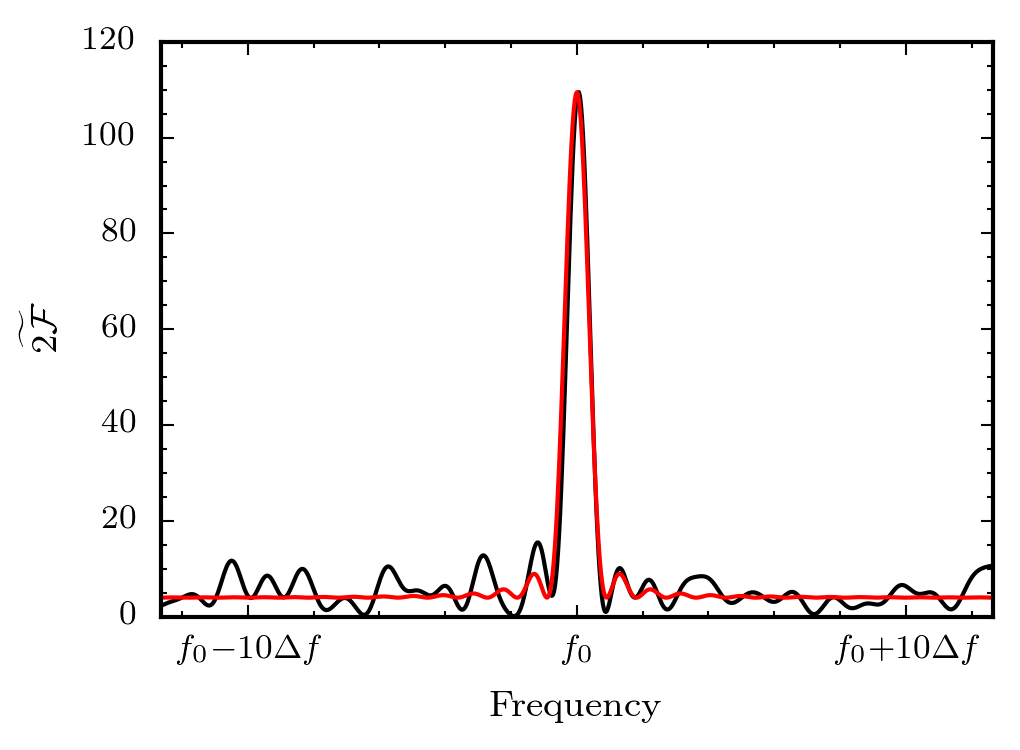
\includegraphics[width=0.45\textwidth]{grided_frequency_search_1D}
\caption{Comparison of the analytic prediction of
Equation~\eqref{eqn_grid_prediction} (in red) with the value computed
numerically from simulating a signal with frequency $f_0$ in Gaussian noise (in
black). $\Delta f$ is the frequency difference corresponding to a
metric-mismatch of unity.}
\label{fig_grid_frequency}
\end{figure}

\subsection{Example: signal in noise}

In order to familiarise the reader with the features of an MCMC search, we will
now describe a simple directed search (over $f$ and $\dot{f}$) for a simulated
signal in Gaussian noise. The signal will have a frequency of
$\BasicExampleFzero$~Hz and a spin-down of $\BasicExampleFone$~Hz/s, all other
Doppler parameters are known and so are irrelevant. Moreover, the signal has an
amplitude $\BasicExamplehzero$~Hz$^{-1/2}$ while the Gaussian noise has
$\sqrt{\Sn}=\BasicExampleSqrtSn$~Hz$^{-1/2}$ such that the signal has a depth
of $\BasicExampleDepth$.

First, we must define a prior for each search parameter Typically, we recommend
either a uniform prior bounding the area of interest, or a normal distribution
centered on the target and with some well defined width. However, to ensure
that the MCMC simulation has a reasonable chance at finding a peak, one should
consider the corresponding metric-volume given in
Equation~\eqref{eqn_metric_volume}. For this example, we will use a uniform
prior with a frequency range of $\Delta f=\BasicExampleDeltaFzero$~Hz and a
spin-down range of $\Delta \fdot=\BasicExampleDeltaFone$~Hz/s both centered on
the simulated signal frequency and spin-down rate. We set the reference time to
coincide with the middle of the data span, therefore the metric volume can be
decomposed into the frequency contribution and spin-down contribution:
frequency,
\begin{align}
\Vpe^{(0)} = \frac{(\pi\Tcoh\Delta f)^2}{3} \approx \BasicExampleVFzero
\end{align}
and
\begin{align}
\Vpe^{(1)} = \frac{4(\pi\Delta \fdot)^2\Tcoh^{4}}{45} \approx \BasicExampleVFone
\end{align}
such that $\V\approx\BasicExampleV$ (note that $\Vsky$ does not contribute
since we do not search over the sky parameters). This metric volume indicates
that the signal will occupy about 1\% of the prior volume, therefore the MCMC
is expected to work. Alternative priors will need careful thought about how to
translate them into a metric volume: for example using a Gaussian one could use
the standard deviation as a proxy for the allowed search region.

In addition to defining the prior, one must also consider how to
\emph{initialise} the walkers. If the prior genuinely represents the stated
prior knowledge, the usual solution is to initialise the walkers from the
prior: that is the starting position is drawn from the prior. However,
instances do occur when one would like to initialise the walkers from a
different distribution. For example, if one only needs to estimate the evidence
(given a particular prior), but is aware from previous searches that the only
significant peak lies in a small area of parameter space, one could initialise
the walkers in a small cluster close to that area. In this example, we
initialise the walkers from the prior such that they have the chance to explore
the entire prior volume.

Having defined the prior, the final setup step is to define the number of
\emph{burn-in} and \emph{production} steps the sampler should take and the
number of walkers; this is a tuning parameter of the MCMC algorithm. The number
of walkers should be typically a few hundred, the greater the number the more
samples will be taken resulting in improved posterior estimates. The burn-in
steps refers to an initial set of steps which are discarded as they are taken
whilst the walkers converge. After they have converged the steps are known as
production steps since they are used to produce posterior estimates and
calculate the marginal likelihood.

Using these choices, the simulation is run. To illustrate the full MCMC
process, in Figure~\ref{fig_MCMC_simple_example} we plot the progress of all
the individual walkers (each represented by an individual line) as a function
of the total number of steps. The red portion of steps are burn-in and hence
discarded, from this plot we see why: the walkers are initialised from the
uniform prior and initially spend some time exploring the whole parameter space
before converging. The fact that they converge to a single unique point is due
to the strength of the signal (substantially elevating the likelihood about
that of Gaussian fluctuations) and the tight prior which was quantified through the
metric volume $\V$. The production samples, colored black, are only taken once
the sampler has converged - these can be used to generate posterior plots.
\begin{figure}[htb]
\centering
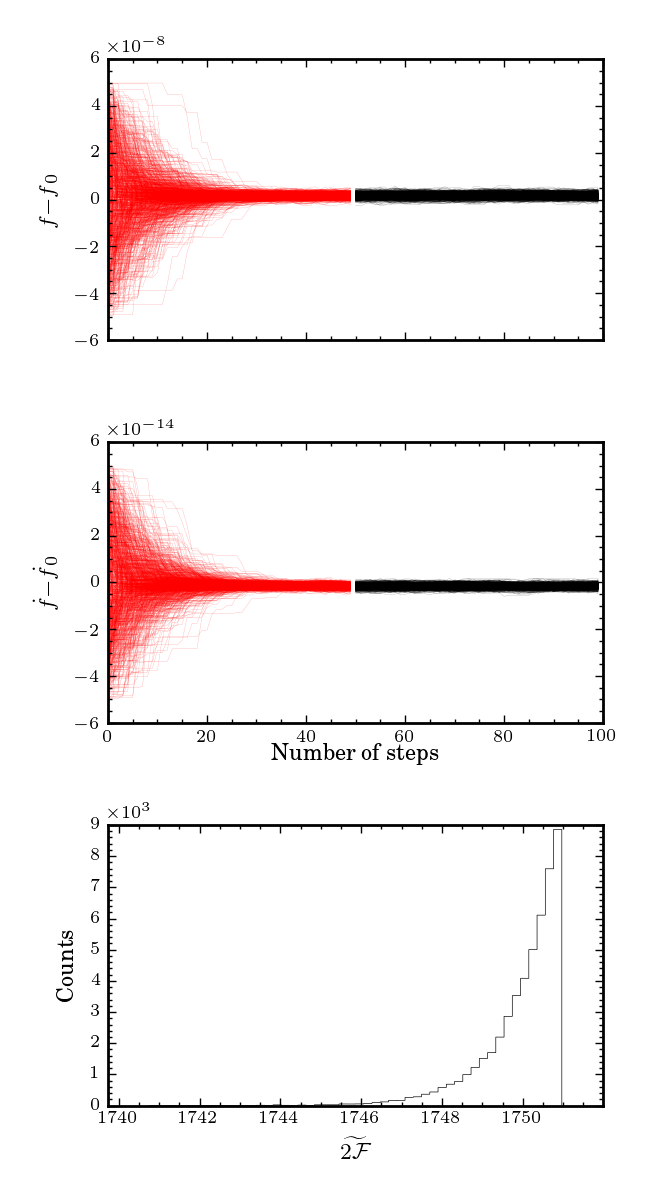
\includegraphics[width=0.45\textwidth]{fully_coherent_search_using_MCMC_walkers}
\caption{The progress of the MCMC simulation for a simulated signal in Gaussian
noise, searching over the frequency and spin-down. The upper two panels show
the position of all walkers as a function of the number of steps for the
frequency and spin-down; when they are colored red the samples are discarded as
burn-in (the first 100 steps), while when they are colored black they are used
as production samples. The bottom panel shows the distribution of
$\widetilde{2\F}$ taken from the production samples.}
\label{fig_MCMC_simple_example}
\end{figure}

\section{Testing convergence}

In Figure~\ref{fig_MCMC_simple_example}, it is easy to see by eye that that the
MCMC simulation has converged during the burn-in. However, choosing the number
of steps, balancing the extra computing cost against ensuring the chains have
converged, is often a matter of trial and error. So, while graphical methods
for assesing convergence are the most robust and informative, quantitative
methods (diagnostics) also exist to test convergence and can therefore provide
the utility to prematurely stop the burn-in period. As such one can then simply
choose a large number of steps (as compared to a typical burn-in for the given
problem) and expect that in most cases these will not all be used. Moreover, if
such a large number of searches are to be run such that inspection of each MCMC
simulation is impossible, the convergence tests can easily be checked
numerically.

\subsection{The Gelman \& Rubin statistic}
We will use the ``Gelman \& Rubin statistic" \citep{gelman1992} to assess
convergence. This method, developed in the context of single-walker samplers
(i.e. not ensemble samplers) requires multiple independent simulations to be
run, each initialised from an overdispersed estimate of the target
distribution. The statistic, the \emph{potential scale reduction factor}
(PSRF), is calculated for each scalar quantity of interest and estimates the
amount by which the scale factor of the target distribition (approximated by a
Student t distribution) might shrink if the simulation where run indefinitely.
This method makes a normality assumption on the posterior distribution, which
in testing appears to be reasonble for all parameters except the transient
start time and durations (discussed later in Sec.~\ref{sec_transients}).
However, paraphrasing \citet{brooks1998}, Gelman and Rubin's approach is
generally applicable to any situation where the posterior inference can be
summarized by the mean and variance (or standard deviation), even if the
posterior distributions are not themselves believed to be normally distributed.

\comment{Note I have not yet fully implemented the method, for simplicity I'm
         assuming df -> infty}

In this setting, we depart from the original description by using the walkers
of the ensemble sampler in place of independent MCMC simulations. Moreover,
this is done periodicically checking the last $n$ steps of the simulation. As
such, testing convergence requires only a small overhead in calculating the
variances: there is no requirement to run multiple independent simulations.
At each periodic check, the statistic is computed for each model parameter
and if all model parameters are less than the threshold (with a default value
of 1.2), the simulation is considered converged. However, the burn-in period is
only prematurely stopped if convergence is reached a pre-specific number of
times (the default value is 10). This is a conservative system to prevent
misdiagnosis of convergence.

While in testing this method was found to agree well with graphical
determination convergence, but we echo the conclusions of \citet{cowles1996markov}
that no convergence diagnostic can say with certainty that the posterior
samples are truly representative of the underlying stationary distribution.

\subsection{Example}

In Figure~\ref{fig_MCMC_convergence_example}, we illustrate our implementation
of the Rubin-Gelman statistic for a fully-coherent search of data including
a strong continuous signal. In essense this repeats the simulation in
Figure~\ref{fig_MCMC_simple_example}, but we have expanded the prior ranges
on $f$ and $\fdot$. As a result, the sampler takes many more steps to reach
convergence: it can be seen by eye that the traces of a few walkers remain
isolated from the bulk of walkers. When this is the case, the PSRF is much
larger than unity, since the between-walker variance is much larger than the
within-walker variance. Once that walker joins the main bulk, the PSRF tends
to unity for several periods and hence the burn-in period is prematurely
halted. The sampler is then continued, with all samples saved as production
samples. In the figure, the gap indicates the `missing' samples which would
have been taken if convergence had not been obtained before the end of the
maximum burn-in period.
\begin{figure}[htb]
\centering
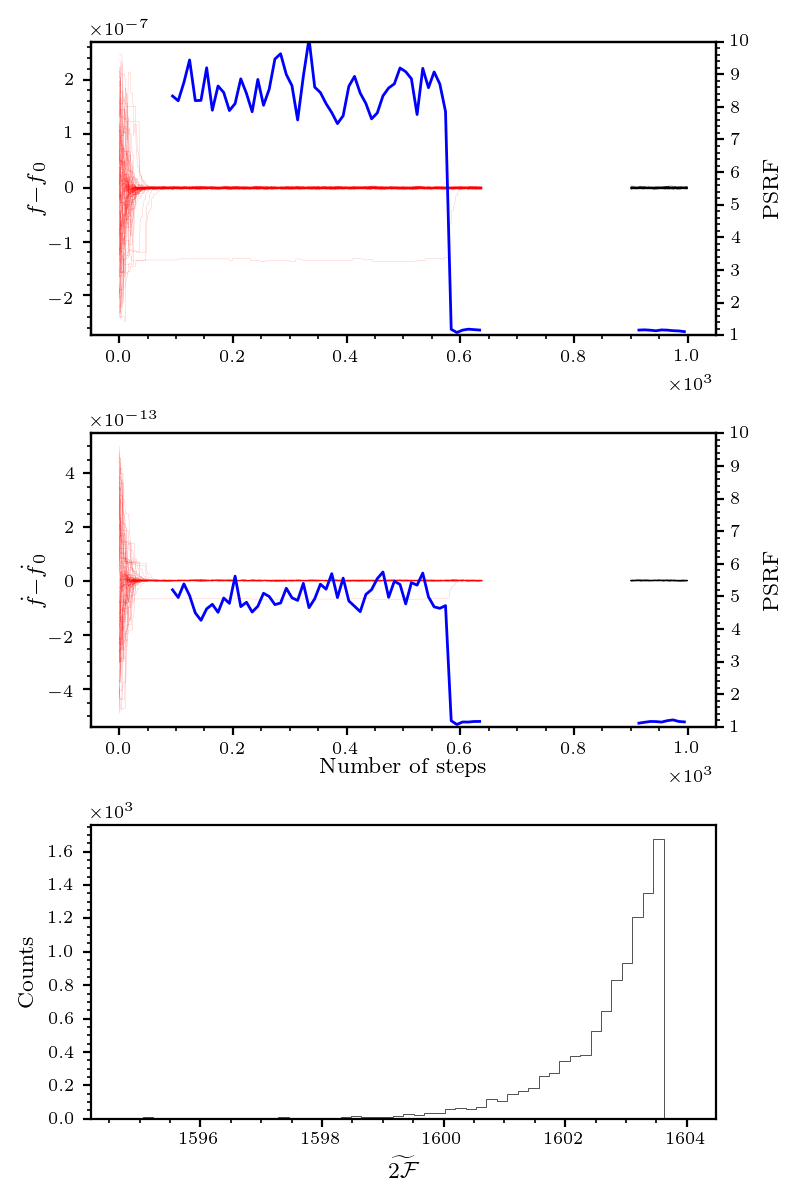
\includegraphics[width=0.5\textwidth]{fully_coherent_search_using_MCMC_convergence_walkers}
\caption{Demonstration of the Potential Scale Reduction Face (PSRF) convergence
statistic (in blue) calculated separately for each parameter: values below 1.2
are considered converged.}
\label{fig_MCMC_convergence_example}
\end{figure}

It is worth noting that this type of long convergence, when a small number of
chains remain isolated from the main bulk can be easily countered by the use
of parallel tempering (see Sec.~\ref{sec_parallel_tempering}). This was intenionally
not used here to highlight the utility of the convergence statistic.


\section{Follow-up}
\label{sec_follow_up}

Incoherent detection statistics trade significance (the height of the peak) for
sensitivity (the width of the peak). We will now discuss the advantages of
using an MCMC sampler to follow-up a candidate found incoherently, increasing
the coherence time until finally estimating its parameters and significance
fully-coherently. We begin by rewriting Equation~\eqref{eqn_lambda_posterior},
the posterior distribution of the Doppler parameters, with the explicit
dependence on the coherence time $\Tcoh$:
\begin{equation}
P(\blambda | \Tcoh, x, \Pic, \Hs, I)
%=\Bsn(x| \Tcoh, \Pic, \blambda) P(\blambda| \Hs I).
\propto e^{\hat{\F}(x| \Tcoh, \blambda)} P(\blambda| \Hs I).
\end{equation}

Introducing the coherent time $\Tcoh$ as a variable provides a free parameter
which adjusts width of signal peaks in the likelihood. Therefore, a natural way
to perform a follow-up is to start the MCMC simulations with a short coherence
time (such that the signal peak occupies a substantial fraction of the prior
volume) and then subsequently incrementally increasing this coherence time in a
controlled manner, aiming to allow the MCMC walkers to converge to the new
likelihood before again increasing the coherence time. Ultimately, this
coherence time will be increased until $\Tcoh = \Tspan$. If this is done in
$\Nstages$ discreet \emph{stages}, this introduces a further set of tuning
parameters, namely the ladder of coherence times $\Tcoh^{i}$, where $i \in [0,
\Nstages]$.

In some ways, this bears a resemblance to `simulated annealing', a method in
which the likelihood is raised to a power (the inverse temperature) and
subsequently `cooled'. The important difference being that the semi-coherent
likelihood is wider at short coherence times, rather than flatter as in the
case of high-temperature simulated annealing stages. For a discussion and
examples of using simulated annealing in the context of CW searches see
\citet{veitch2007}.

Of course in practice, we can't arbitrarily vary $\Tcoh^i$, but rather the
number of segments at each stage $\Nseg^{i}\equiv \Tspan/\Tcoh^{i} \in
\mathbb{N}$.  Ideally, the ladder of segment should be chosen to ensure that
the metric volume at the $i^{th}$ stage $\V_i \equiv \V(\Nseg^i)$ is a constant
fraction of the volume at adjacent stages. That is we define
\begin{equation}
\mathcal{R} \equiv \frac{\V_i}{\V_{i+1}},
\end{equation}
where $\mathcal{R} \ge 1$ as $\Tcoh^{i+1} > \Tcoh^{i}$.

For the MCMC simulations to be succesful, this initial bounding
box, given the segment setup which produced the candidate, must be small
compared to the width of the signal (at that segment setup). If we start out
follow-up with the same search setup used in the source search, i.e.  we set
$\Nseg^0$ equal to the number of segments used in the input search, then for
the MCMC simulation to work, we require that $\V(\Nseg^{0}) \sim \mathcal{O}(100)$.

Given a fixed prior on the Doppler parameters and a fixed span of data, the
metric volume $\V_{\Nstages}$ for $\Tcoh^{\Nstages} = \Tspan$ is fixed, or in
terms of the number of segments, $\Nseg^{\Nstages} = 1$.
We can therefore define a minimisation problem:
\begin{align}
\min_{\Nseg^{i+1} \in \mathbb{N}}
\left| \log\mathcal{R} + \log\V(\Nseg^{i+1}) - \log\V(\Nseg^i)\right|
\end{align}
which can be solved numerically to a specified tolerance. Due to the difficulty
in solving such a minimisation with the integer constrain on $\Nseg^{i+1}$ we
simply solve it as a real scalar, and then round to the nearest integer. We now
have a method to generate a ladder of $\Nseg^{i}$ which keep the ratio of
volume fractions fixed. Starting with $\Nseg^{\Nstages}$ = 1, we generate
$\Nseg^{\Nstages-1}$ such that $\V^{\Nstages-1} < \V^{\Nstages}$ and
subsequently iterate.  Finally we must define $\V^{\rm min}$ as the stopping
criterion: a metric volume such that the initial stage will find a signal. This
stopping criterion itself will set $\Nstages$; alternatively one could set
$\Nstages$.

We have now defined a method to automate the task of choosing the ladder of
coherence times. This requires only two tuning parameters, the ratio between
stages $\mathcal{R}$ and the minimum metric volume $\V^{\min}$.

\subsection{Example}

We now provide an illustrative example of the follow-up method. We consider a
directed search over the sky position and frequency in 100 days of data from a
single detector, with $\sqrt{\Sn}=10^{-23}$~Hz$^{-1/2}$ (at the fiducial
frequency of the signal). The simulated signal has an amplitude
$h_0=2\times10^{-25}$ such that the signal has a depth of $\sqrt{\Sn}/h_0=50$
in the noise.

First, we must define the setup for the run. Using $\mathcal{R}=10$ and
$\V^{\rm min}=100$ our optimisation procedure is run and proposes the setup
layed out in Table~\ref{tab_follow_up_run_setup}. In addition, we show the
number of steps taken at each stage.
\begin{table}[htb]
\caption{The search setup used in Figure~\ref{fig_follow_up}, generated with
$\mathcal{R}=10$ and $\V^{\rm min}=100$.}
\label{tab_follow_up_run_setup}
\begin{tabular}{c|cccccc}
Stage & $\Nseg$ & $\Tcoh^{\rm days}$ &$\Nsteps$ & $\V$ & $\Vsky$ & $\Vpe$ \\ \hline
0 & 100 & 1.0 & 200 & 95.0 & 6.8 & 14.0 \\
1 & 56 & 1.8 & 200 & $9.6{\times}10^{2}$ & 22.0 & 45.0 \\
2 & 31 & 3.2 & 200 & $1.0{\times}10^{4}$ & 69.0 & $1.5{\times}10^{2}$ \\
3 & 17 & 5.9 & 200 & $1.1{\times}10^{5}$ & $2.3{\times}10^{2}$ & $4.8{\times}10^{2}$ \\
4 & 9 & 11.1 & 200 & $1.3{\times}10^{6}$ & $7.5{\times}10^{2}$ & $1.7{\times}10^{3}$ \\
5 & 5 & 20.0 & 200 & $1.1{\times}10^{7}$ & $2.0{\times}10^{3}$ & $5.5{\times}10^{3}$ \\
6 & 2 & 50.0 & 200 & $1.0{\times}10^{8}$ & $3.3{\times}10^{3}$ & $3.1{\times}10^{4}$ \\
7 & 1 & 100.0 & 200,200 & $2.7{\times}10^{8}$ & $4.4{\times}10^{3}$ & $6.2{\times}10^{4}$ \\
\end{tabular}

\end{table}

The choice of $\mathcal{R}$ and $\V^{\rm min}$ is a compromise between the
total computing time and the ability to ensure a candidate will be identified.
From experimentation, we find that $\V^{\rm min}$ values of 100 or so are
sufficient to ensure that any peaks are sufficiently broad during the
initial stage. For $\mathcal{R}$ value much larger than $10^{3}$ or so where
found to result in the MCMC simulations `loosing' the peaks between stages, we
conservatively opt for 10 here, but values as large as 100 where also successful.

In Figure~\ref{fig_follow_up} we show the progress of the MCMC sampler during
the follow-up.  As expected from Table~\ref{tab_follow_up_run_setup}, during
the initial stage the signal peak is broad with respect to the size of the
prior volume, therefore the MCMC simulation quickly converges to it. Subsequently,
each time the number of segments is reduced, the peak narrows and the samplers
similarly converge to this new solution. At times it can appear to be inconsistent,
however this is due to the changing way that the Gaussian noise adds to the signal.
Eventually, the walkers all converge to the true signal.
\begin{figure}[htb]
\centering
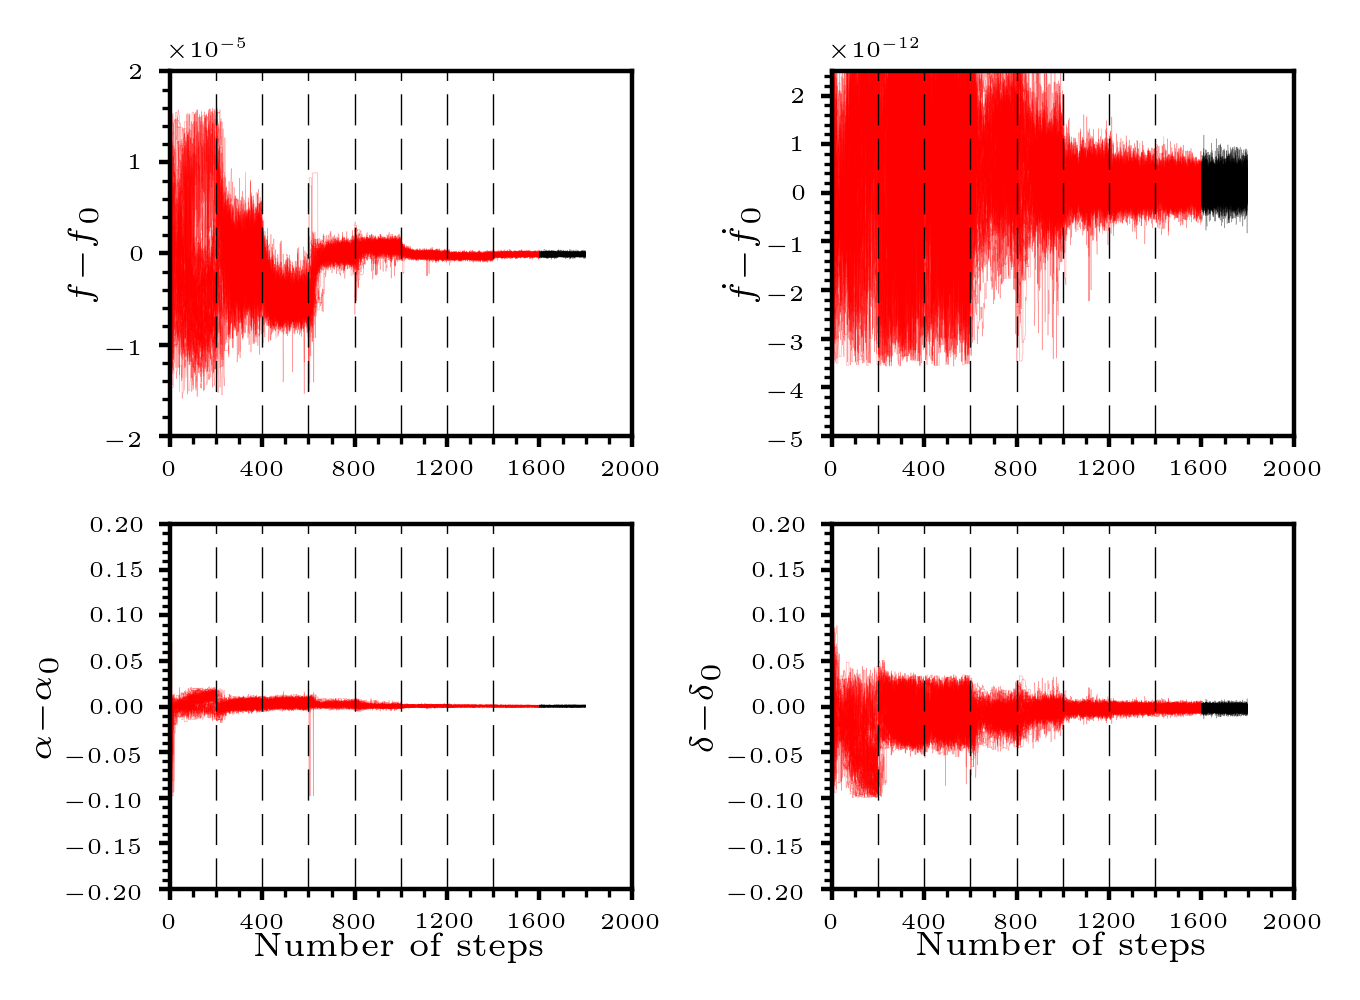
\includegraphics[width=0.5\textwidth]{follow_up_walkers}
\caption{In the top three panels we show the progress of the 500 parallel
walkers (see Figure~\ref{fig_MCMC_simple_example} for a description) during the
MCMC simulation for each of the search parameters, frequency $f$,
right-ascension $\alpha$ and declination $\delta$. Each vertical dashed line indicates the start of a new stage of the search, the parameters for all stages
are listed in Table~\ref{tab_follow_up_run_setup}.}
\label{fig_follow_up}
\end{figure}

The key advantage to note here is that all walkers successfully converged to the
signal peak, which occupies $\sim 10^{-6}$ of the initial volume. While it is
possible for this to occur during an ordinary MCMC simulation (with $\Tcoh$
fixed at $\Tspan$), it would take substantially longer to converge as the
chains explore the other `noise peaks' in the data.

\section{Monte Carlo studies}

In order to understand how well the MCMC follow-up method works, we will test
its ability to succesfully identify simulated signals in Gaussian noise. This will be
done in a Monte Carlo study, with independent random realisations of the
Guassian noise, amplitude, and Doppler parameters in suitable ranges. Such a
method is analagous to the studies performed in \citet{shaltev2013}, except
that we present results as a function of the fixed injected signal depth,
rather than the squared SNR.

In particular we will generate a number of 100-day data sets containing
independent realisations of Gaussian noise and a simulated CW signal. We choose
the parameters of the signal in such a way to model the candidates generated
from directed and all-sky searches by drawing the signal parameters from
appropriate distributions. However, we do not draw $h_0$ randomly, but instead
run the MC study at a number of selected values chosen such that given the
fixed $\sqrt{S_n}=1\times10^{3}$, the signals are injected with a depth
$\mathcal{D} \in [100, 400]$.  To simulate an isotropic distribution of
sources, we draw the remaining amplitude parameters for each signal uniformly
from $\phi \in [0, 2\pi]$, $\psi \in [-\pi/4, \pi/4]$, and $\cos\iota \in [-1,
1]$.

To provide a reference, we will compare the MC follow-up study against the
expected maximum theoretical detection probability for an infinitly dense
fully-coherent search of data containing isotropically-distributed signals as
calculated by \citet{wette2012}. Note however that we will parameterise with
respect to the signal depth (i.e. using Equation~(3.8) of \citet{wette2012} to
relate the averaged-SNR to the depth). The probability is maximal in the
sense that signals are `lost' during the follow-up due simply to the fact that
they are not sufficiently strong to rise above the noise.


\subsection{Follow-up candidates from a directed search}
\label{sec_directed_follow_up}

In a directed search, the sky location parameters $\alpha$ and $\delta$ are
fixed - in our study we fix them on the location of the Crab pulsar, but this
choice is arbitrary and holds no particular significance. The ouput of a
semi-coherent gridded directed search would provide the grid-point with the
highest detection statistic, and some box bounding the candidate given some
uncertainty. We will assume in this section that given the search setup
$\Nseg^{0}$ of the input search, the bounding box is sufficiently small to
ensure that $\V(\Nseg^0)\sim \mathcal{O}(100)$. This is not a limiting
assumption as any search can (quite cheaply) increase the density of grid
points around any interesting candidates in order to better constrain their
uncertainty.

Before applying the directed follow-up to simulated signals in noise, we need
to characterise its behaviour in Gaussian noise alone. To do so, we simulate
$\DirectedMCNoiseN$ realisations of Gaussian noise and peform the follow-up
search on these. A histogram of the results is provided in
Figure~\ref{fig_hist_DirectedMCNoiseOnly}, the largest observed value was
found to be $\DirectedMCNoiseOnlyMaximum$. From this, we can set a threshold
for the detection statistic of $\twoFtilde_{\rm th} = 60$, an arbitrary
number chosen to be sufficiently larger than the maximum seen in noise and
consistent with the value chosen in \citet{shaltev2013}.
\begin{figure}[htb]
\centering
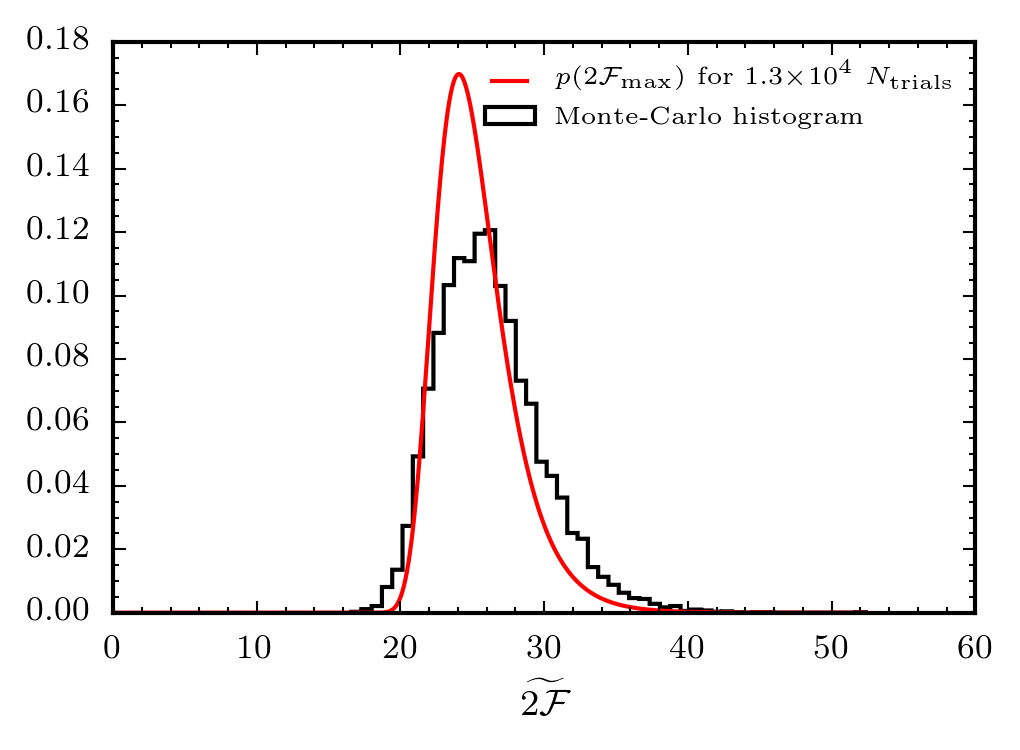
\includegraphics[width=0.5\textwidth]{directed_noise_twoF_histogram}
\caption{Histogram of the recovered $\widetilde{2\F}$ values applying the
directed follow-up routine to $\DirectedMCNoiseN$ simulated Gaussian noise
realisations.}
\label{fig_hist_DirectedMCNoiseOnly}
\end{figure}

The behaviour of the follow-up is independent of the exact frequency and
spin-down values used (this is not true for an all-sky follow-up as discussed
in Section~\ref{sec_all_sky_follow_up}). As such, we can, without loss of
generality define our Monte-Carlo follow-up in the following way. First, we
select an arbitrary frequency and spindown of $f_0=30$~Hz and
$\dot{f}_0=10^{-10}$Hz/s and a surrounding uncertainty box $\Delta f$ and
$\Delta \dot{f}$ chosen such that the uncertainty in frequency and spindown are
roughly equivalent in terms of mismatch. Then, we pick a candidate uniformly
from within this uncertainty box; this choice reflects the fact that the grid
is chosen such that the probability distribution of candidate signals is
uniform.

Having generated the data given the prescription above, we proceed to perform a
hierarchical MCMC follow-up. Given the data span and initial bounding box, we
compute the optimal heirarchical setup, the details of which are given in
Table~\ref{tab_directed_MC_follow_up}, this setup was used for all MC
simulations. This table also lists the number of steps, which in this case we
chose to be 10 - quite a small number of steps for a typical MCMC simulation.

\begin{table}[htb]
\caption{Run-setup for the directed follow-up Monte-Carlo study, generated with
$\mathcal{R}=10$ and $\Nseg^0=20$.}
\label{tab_directed_MC_follow_up}
\begin{tabular}{c|cccc}
Stage & $\Nseg$ & $\Tcoh^{\rm days}$ &$\Nsteps$ & $\Vpe$ \\ \hline
0 & 20 & 5.0 & 25 & 60.0 \\
1 & 7 & 14.3 & 25 & $5{\times}10^{2}$ \\
2 & 2 & 50.0 & 25 & $5{\times}10^{3}$ \\
3 & 1 & 100.0 & 25,25 & $1{\times}10^{4}$ \\
\end{tabular}

\end{table}

This process yeilds a maximum detection statistic $\widetilde{2\F}_{\rm max}$.
The signal is considered `detected' if $\widetilde{2\F}^{\rm max} >
\widetilde{2\F}_{\rm th}$, where we set the threshold at $2\F_{\rm th}=60$. In
Figure~\ref{fig_directed_MC_follow_up} we plot the the fraction of the MC
simulations which where recovered and compare this against the theoretical
maximum, given the threshold. The figure demonstrates that the recovery power
of the MCMC follow-up shows only a small margin of loss compared to the
theoretical maximum. \comment{Probably best to run with more steps and see if
this doesn't remove the loss}
\begin{figure}[htb]
\centering
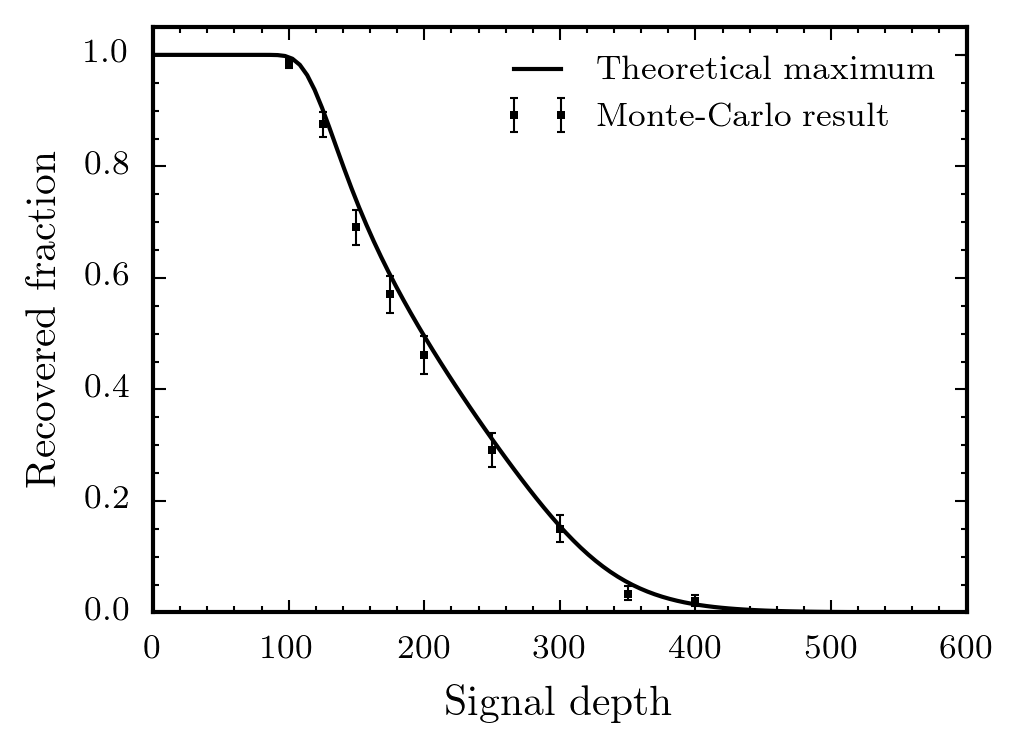
\includegraphics[width=0.45\textwidth]{directed_recovery}
\caption{Recovery fraction for the directed follow-up. The Monte-Carlo results
come from random draws searches using the setup described in
Table~\ref{tab_directed_MC_follow_up}.}
\label{fig_directed_MC_follow_up}
\end{figure}


\subsection{Follow-up candidates from an all-sky search}
\label{sec_all_sky_follow_up}

We now test the follow-up method when applied to candidates from an all-sky
search which, by definition, have uncertain sky-position parameters $\alpha$
and $\delta$. Searching over these parameters, in addition to the frequency
and spin-down not only increases the parameter space volume that needs to be
searched, but also adds difficulty due to correlations between the sky-position
and spin-down \comment{Does some of Karl's work discuss this?}.

To replicate the condition of candidates from an all-sky search, we draw the
candidate positions isotropically from the unit sphere (i.e. $\alpha$ uniform
on $[0, 2\pi]$ and $\delta = \cos^{-1}(2u{-}1){- }\pi/2$ where $u$ is uniform
on $[0, 1]$). We then place an uncertainty box containing the candidates with a
width $\Delta\alpha=\Delta\delta=0.05$; this box is not centered on the
candidate, but chosen in such a way that the location of the candidate has a
uniform probability distrubution within the box. This neglects the non-uniform
variation in $\delta$ over the sky-pacth, but given the small area should not
cause any significant bias. The frequency, spin-down, and amplitude parameters
are chosen in the same way as for the directed search
(Section~\ref{sec_directed_follow_up}). 

Again, we first characterise the behaviour of the all-sky follow-up by applying
it to $\AllSkyMCNoiseN$ realisations of Gaussian noise. The resulting histogram
is provided in Figure~\ref{fig_hist_AllSkyMCNoiseOnly} and the largest $\twoFtilde$
value was found to be $\AllSkyMCNoiseOnlyMaximum$. This is larger than the
value found for the directed search, although both use the same number of
Gaussian noise trials, and therefore must result from the increased number of
search parameters. \comment{Ask Reinhard about Miroslavs statement on number of
templates}. As a result we will correspondinly increase our detection threshold
for the all-sky search to $\twoFtilde_{\rm tr} = 70$; again this is an arbitary
choise, but is consisent with the values chosen in \citet{shaltev2013}.
\begin{figure}[htb]
\centering
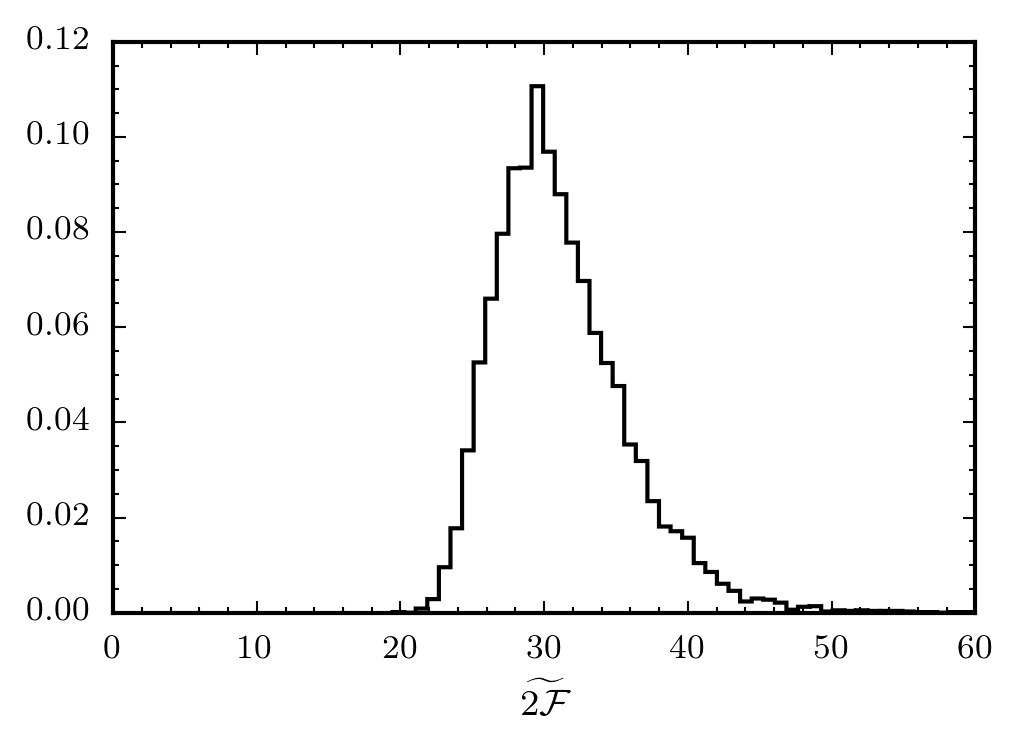
\includegraphics[width=0.5\textwidth]{allsky_noise_twoF_histogram}
\caption{Histogram of the recovered $\widetilde{2\F}$ values applying the
all-sky follow-up routine to $\AllSkyMCNoiseN$ simulated Gaussian noise
realisations.}
\label{fig:}
\end{figure}

Producing \CHECK{1000} indepedant MC simulations we the perform a follow-up on
each using the setup given in Table~\ref{tab_allsky_MC_follow_up}. The
resulting recovery fraction as a function of the injected signal depth is given
in Figure~\ref{fig_allsky_MC_follow_up}.

\begin{table}[htb]
\caption{Run-setup for the all-sky follow-up Monte-Carlo study, generated with
$\mathcal{R}=10$ and $\Nseg^0=20$. Note that the number of representative
templates will vary over the sky, these values are computed at the equator
(i.e. $\delta=0$) which was found to produce the largest volumes - potentially
because the sky patch is kept constant.}
\label{tab_allsky_MC_follow_up}
\begin{tabular}{c|cccccc}
Stage & $\Nseg$ & $\Tcoh^{\rm days}$ &$\Nsteps$ & $\V$ & $\Vsky$ & $\Vpe$ \\ \hline
0 & 20 & 5.0 & 50 & $2{\times}10^{2}$ & 10.0 & 10.0 \\
1 & 11 & 9.1 & 50 & $2{\times}10^{3}$ & 40.0 & 50.0 \\
2 & 6 & 16.7 & 50 & $2{\times}10^{4}$ & $1{\times}10^{2}$ & $2{\times}10^{2}$ \\
3 & 3 & 33.3 & 50 & $1{\times}10^{5}$ & $2{\times}10^{2}$ & $6{\times}10^{2}$ \\
4 & 1 & 100.0 & 50,50 & $8{\times}10^{5}$ & $3{\times}10^{2}$ & $2{\times}10^{3}$ \\
\end{tabular}

\end{table}

\begin{figure}[htb]
\centering
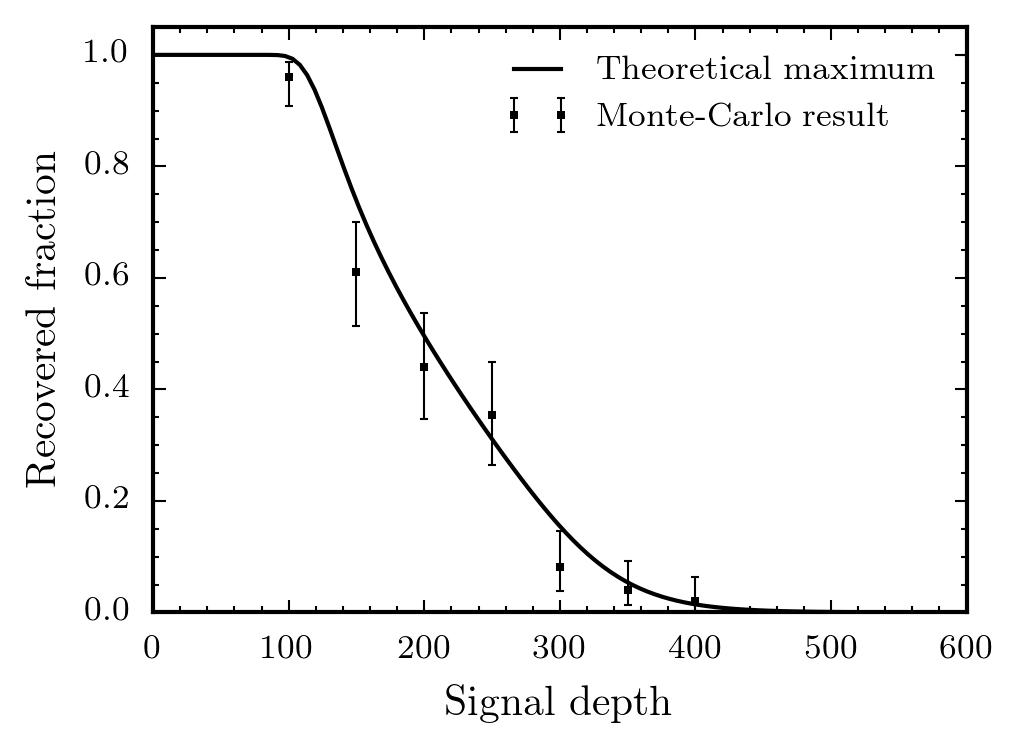
\includegraphics[width=0.45\textwidth]{allsky_recovery}
\caption{Recovery fraction for the all-sky follow-up. The Monte-Carlo results
come from random draws searches using the setup described in
Table~\ref{tab_directed_MC_follow_up}.}
\label{fig_allsky_MC_follow_up}
\end{figure}

\section{Alternative waveform models}

In a grided search, the template bank is constructed to ensure that a canonical
CW signal (i.e. when it lasts much longer than the observation span and has a
phase evolution well-described by a Equation~\eqref{eqn_phi}) will be
recovered with a fixed maximum loss of detection statistic; this loss can be
described as the `template-bank mismatch'. In addition to this mismatch, CW
searches may experience a mismatch if the waveform model differs from the
matched-filter template. There are of course an unlimited number of ways this
may manifest given our ignorance of neutron stars, but from studying pulsars
three obvious mechanisms present themselves: transient, glitching, and noisy
waveforms. In the following sections we will discuss the first two of these, we
discussed the effect of random jitters in the phase evolution (noisy waveforms)
in \citet{ashton2015} and concluded it was unlikely to be of immediate concern.

\subsection{Transients}
\label{sec_transients}

The term \emph{transient-CWs} refers to periodic gravitational wave signals
with a duration $\mathcal{O}(\textrm{hours-weeks})$ which have a
phase-evolution described by Equation~\eqref{eqn_phi}. \citet{prix2011} coined
this term and layed out the motivations for searching for such signals: in
essence it is astrophysically plausible for each signals to exist and we should
therefore build tools capable of finding them. Moreover, the authors described
a simple extension to the $\F$-statistic (and by inheritance to all associated
detection statistics) which provides a method to search for them. This
introduces three new parameters, the start time, duration and a window-function
which determines the evolution of $h_0(t)$ (typical examples being either a
rectangular window or an exponential decay). These methods are implemented in
the code-base used by our sampler to compute the likelihood and therefore we
can expose these search parameters to our MCMC optimisation. In the following
we will detail a simple example showing when it may be appropriate to search for
a transient signal and how it is handles by the MCMC sampler.

We simulate a signal in Gaussian noise at a depth of 10. If the signal where to
be continuous (i.e. last for the entire duration of the data span), it should
be recovered with a predicted detection statistic of
$\widetilde{2\F}\approx5162$. However, the signal we inject is transient in
that it start one third of the way through the data span and stops abruptly
two-thirds of the of the way through (with a constant $h_0$ during this
period). Since the signal lasts for only $1/3$ of the original data span, the
expected $\widetilde{2\F}$ of the transient signal in a matched-filter over only
the portion of data for which it is `on' is $5162/3\approx1720$.

Running a fully-coherent MCMC search over the whole data span, we find a peak
in the likelihood, but with a detection statistic of $\widetilde{2\F}=596$;
this equates to a mismatch of $\approx0.9$: we have lost more significance due
to the inclusion of noise-only data into the matched filter.

In a real search, we cannot know beforehand what the $h_0$ of the signal will
be, so it is not possible to diagnose that the signal is transient due to this
mismatch. However, there does exist tools which can help in this regard. In
this case, plotting the cumulative $\widetilde{2\F}$, as shown in
Figure~\ref{fig_transient_cumulative_twoF}, demonstrates that the first 100
days contributes no power to the detection statistic, during the middle 100
days there is an approximately linear increasing in $\widetilde{2\F}$ with time
(as expected for a signal), while in the last 100 days this is a gradual decay
from the peak. Such a figure is characteristic of a transient signal.
\begin{figure}[htb]
\centering
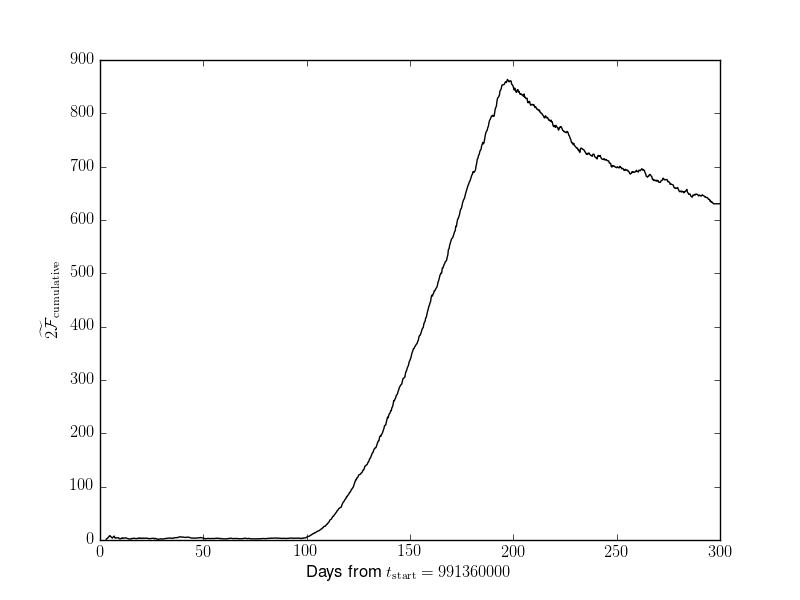
\includegraphics[width=0.45\textwidth]{transient_search_initial_stage_twoFcumulative}
\caption{Plot of the cumulative $\widetilde{2\F}$ for a transient signal with a
constant $h_0$ which lasts from 100 to 200 days from the observation start
time.}
\label{fig_transient_cumulative_twoF}
\end{figure}

Having identified that the putative signal may fact be transient, an extension
of the follow-up procedure is to search for these transient parameters. In our
MCMC method, these require a prior. For the window-function, one must define it
either to be rectangular or exponential: one could run both and then use the
estimated Bayes factors to decide between the two priors. For the start-time it
is sufficient to provide a uniform distribution on the observation span, the
duration can similarly be chosen as a uniform distribution from zero to the
total observation span, or more informatively the absolute value of a central
normal distribution placing greater weight on shorter transients. The choice of
prior can allow the transient signal to overlap with epochs outside of the data
span, in such instances if the likelihood can be computed they are allowed, but
if the likelihood fails (for example if there is no data) the likelihood is
returns as $-\infty$. Putting all this together, we run the sampler on the
simulated transient signal and obtain the posterior estimates given in
Figure~\ref{fig_transient_posterior}. The resulting best-fit has a
$\widetilde{2\F}\approx 1670$, in line with the expected value. Comparing the
Bayes factors between the transient and fully-coherent search can quantify if
the improvement in fit due to the inclustion of the transient parameters was
sufficient to compensate for the greater prior volume and produce an
improvement in the evidence for the model.

\begin{figure}[htb]
\centering
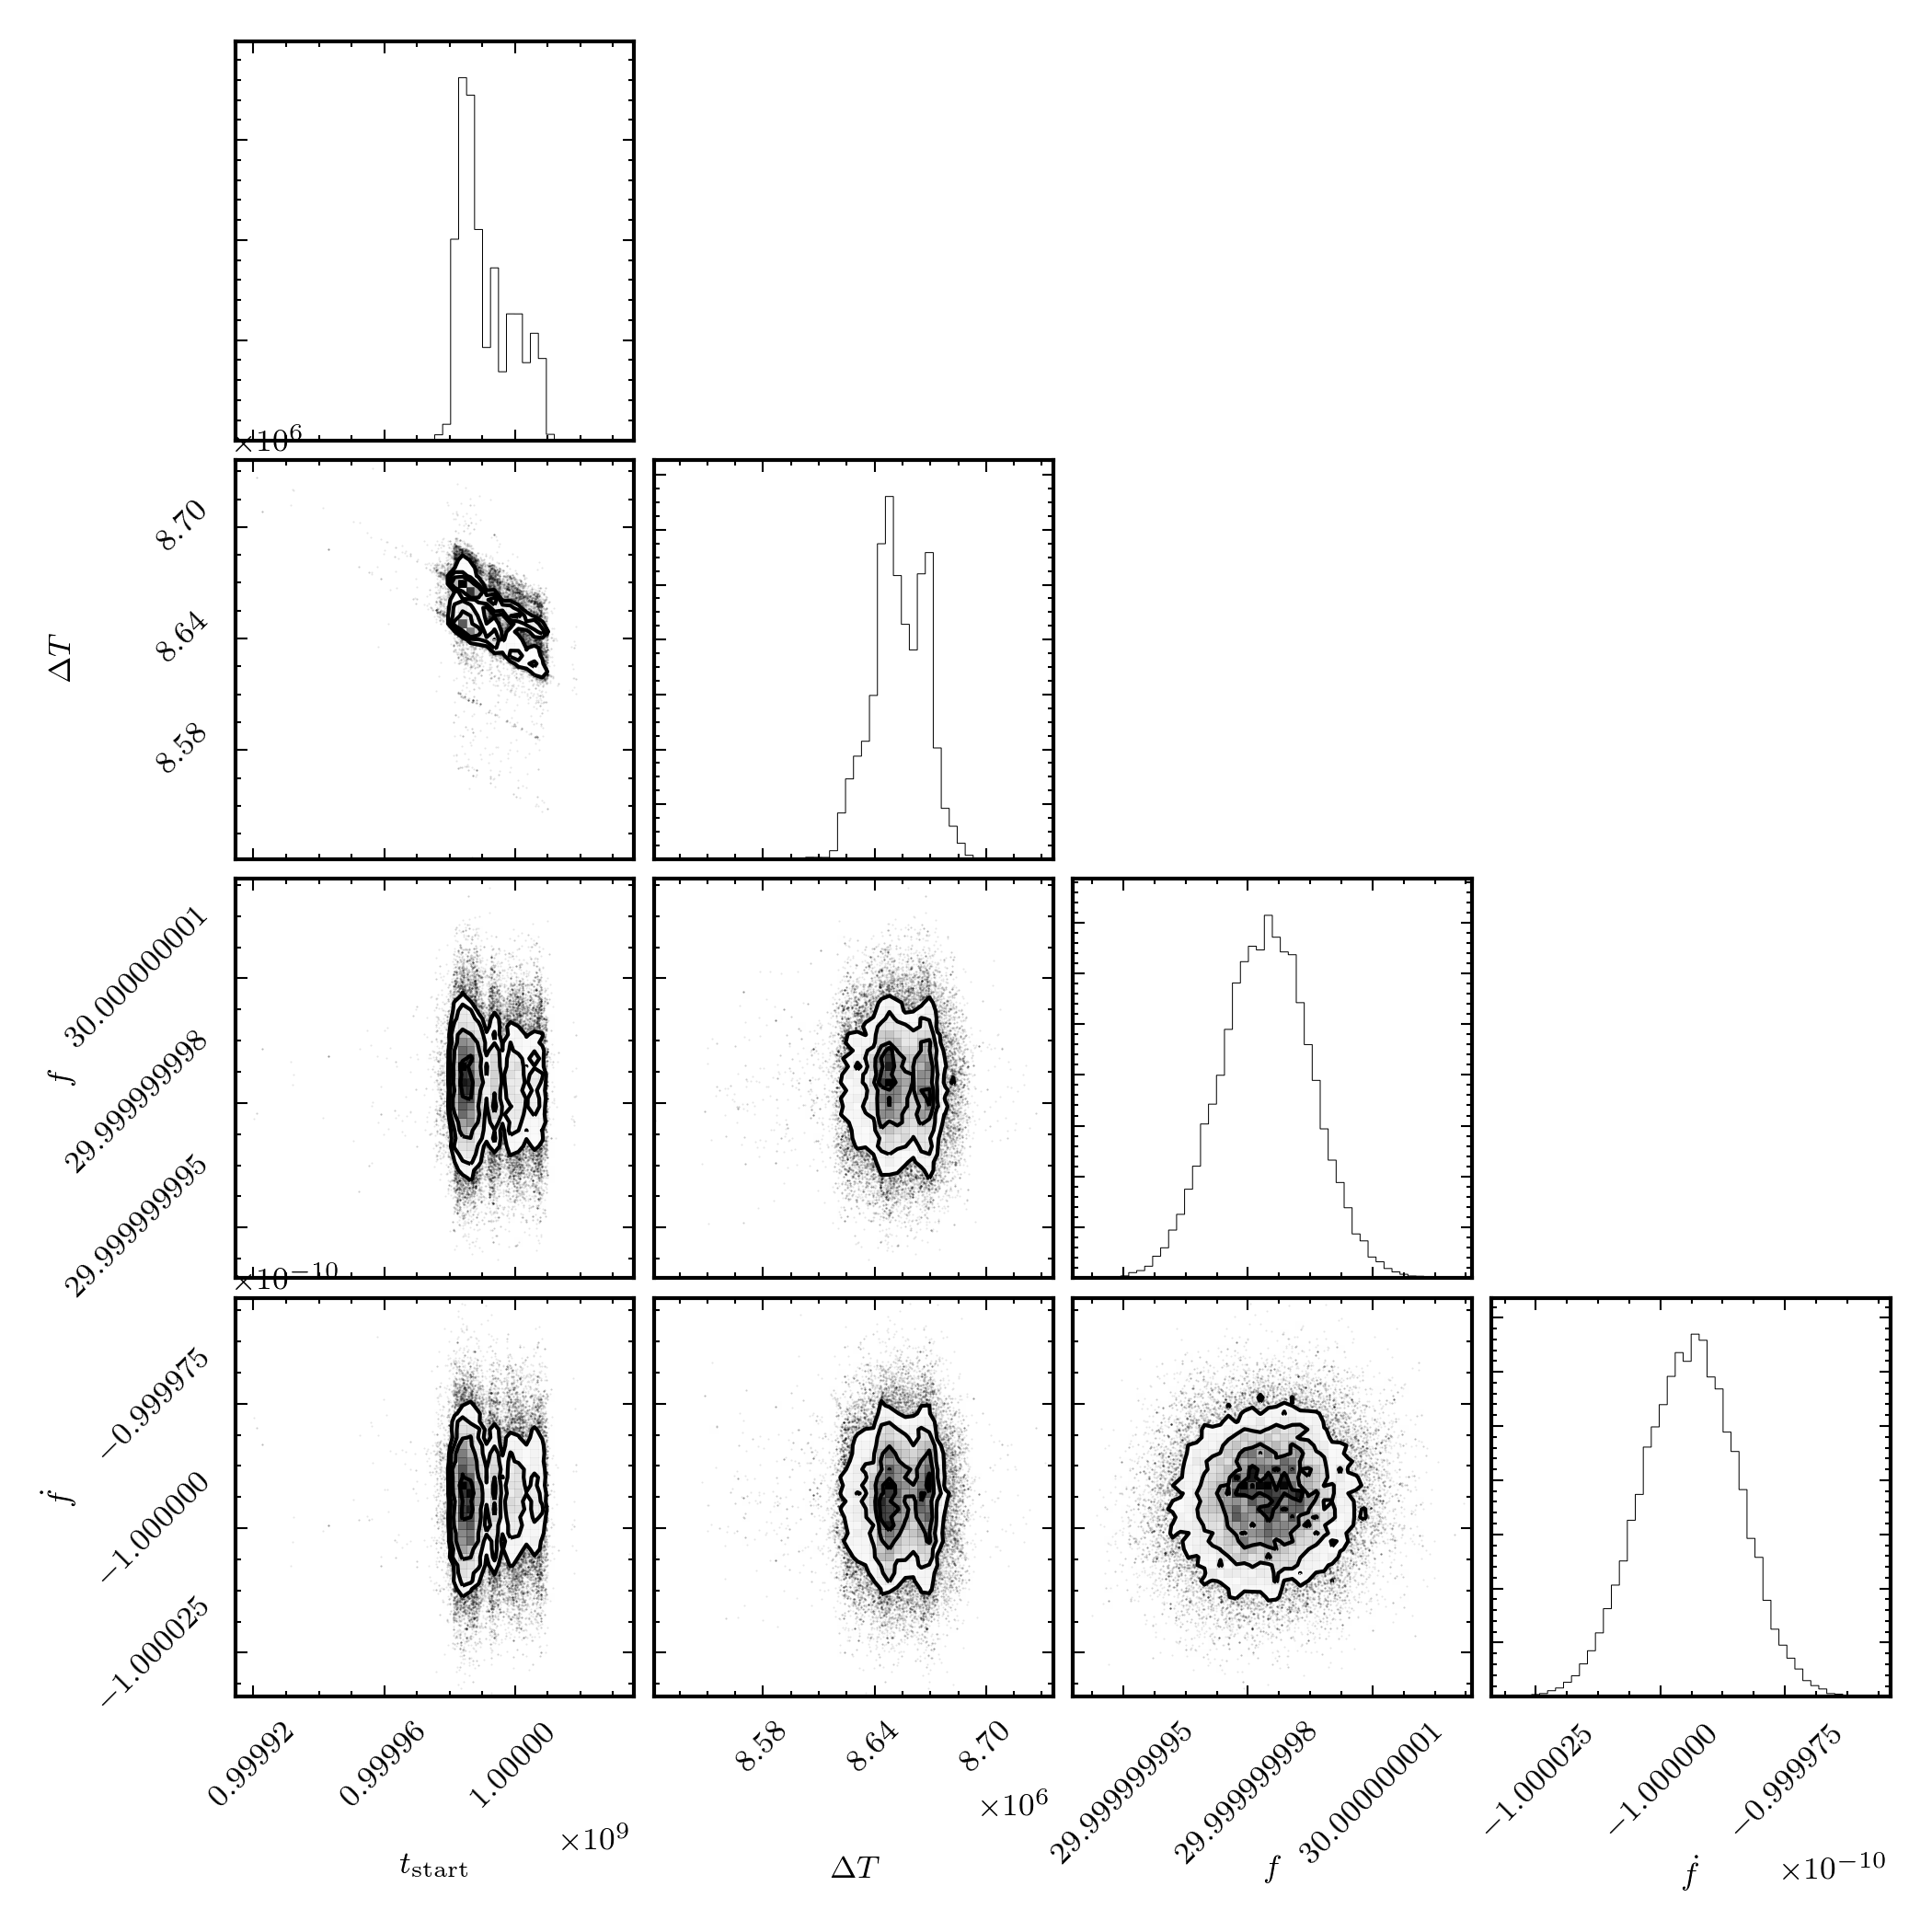
\includegraphics[width=0.45\textwidth]{transient_search_corner}
\caption{Posterior distributions for a targeted search of data containing
a simulated transient signal and Gaussian noise.}
\label{fig_transient_posterior}
\end{figure}



\subsection{Glitches}
\label{sec_glitches}

Observations of radio pulsars show that occasionally neutron stars undergo
sudden glitch events during which the pulsation frequency suddenly
\emph{increases} quite distinct from the usual spin-down due to EM or GW
torques (see \citet{espinoza2011} for a review). These events are typically
Poisson distributed \citet{melatos2008}, but the exact mechanism is not yet
fully understood. However, it seems plausible that the glitch mechanism will
similarly effect any CW emission, i.e. CW signals will also undergo glitches.
In \citet{ashton2016} we demonstrated that if this is the case, CW sources in
directed and all-sky searches have a reasonable probability of undergoing one
or more glitches during typical observations spans and that these glitches may
be sufficiently large to disrupt the detection; this is particuarly true for
areas of parameter space with large spindowns. However, the effect is mitigated
by the use of incoherent searches. As such, we may expect all-sky and directed
searches to correctly identify glitching signals as candidates, but
subseuqnetly `loose' them during the follow-up process. As such, we will now
discuss how the $\F$-statistic optimisation routine discussed in this work can
be used to search for glitching signals.

We will model a glitch as a sudden discontinuous change in the  Doppler
parameters $\delta \blambda$ at some time $\tglitch$: that the change is only
in the frequency and spin-down Doppler parameters, i.e. $\delta\blambda = [0,
0, \delta f, \delta \fdot, \ldots]$. This is to be interpretted, as is done for
radio-pulsar glitches, as the instantaneous change in frequency and spindown at
the time of the glitch. Moreover, multiple glitches can be included (we will
define $\Nglitches$ as the number of glitches) by adding
an index to the glitch magnitude and glitch time.

An ideal glitch search would include these new parameters into the phase model
itself and compute the $\F$-statistic fully-coherently i.e. rewriting
Equation~\eqref{eqn_B_S_N} as
\begin{multline}
\Bsn(x| \tglitch, \delta\blambda, \Pic, \blambda, I) \equiv \\
\int
\mathcal{L}(x ;\A, \blambda, \tglitch, \delta\blambda)
P(\A| \Hs, I) d\A
\end{multline}
where $\tglitch, \delta\blambda$ modify the phase model. However, we propose the
following pragmatic approach: let us instead use an semi-coherent detection
statistic with the epoch between \emph{segments} as $\tglitch$, i.e.
\begin{multline}
\Bsn(x| \tglitch, \delta\blambda, \Pic, \blambda, I) \equiv \\
\int_{\tstart}^{\tglitch}
\mathcal{L}(x ;\A, \blambda)
P(\A| \Hs, I) d\A \\ +
\int_{\tglitch}^{\tend}
\mathcal{L}(x ;\A, \blambda{+}\delta\blambda)
P(\A| \Hs, I) d\A
\end{multline}

This simplistic method leverages readily available and tested code with a loss
of sensitivity over the fully-coherent search by a factor
$\sqrt{\Nglitches+1}$. Such a loss is acceptable, given that the signals must
be sufficiently strong to have been identified by the initial all-sky or directed
search.

As an illustration of the use of this method, we simulate a signal in Gaussian
noise which undergoes a glitch. Firstly in Figure~\ref{fig_glitch_grid} we show
the fully-coherent $2\F$ value computed for a grid of points: this distinctly
shows two peaks, a feature indicative of a glitching signal, with a maximum
value of $\sim\CHECK{400}$. Using our incoherent glitch statistic, we plot
the resulting posterior distributions in Figure~\ref{fig_glitch_posteriors}.

\begin{figure}[htb]
\centering
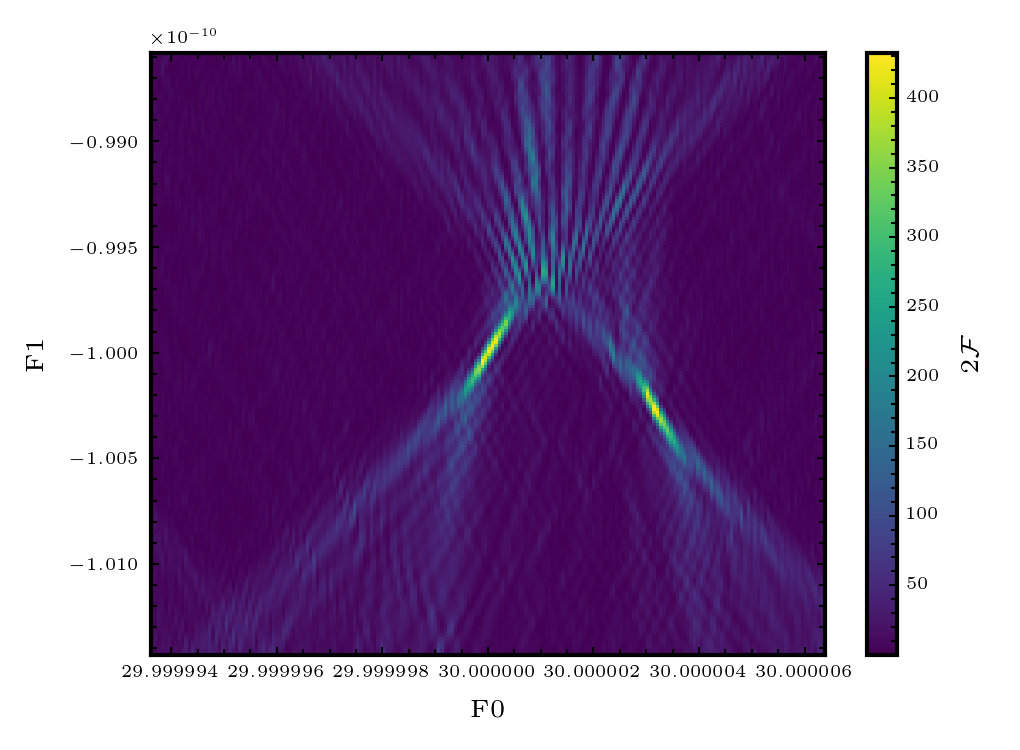
\includegraphics[width=0.5\textwidth]{single_glitch_F0F1_grid_2D}
\caption{}
\label{fig_glitch_grid}
\end{figure}

\begin{figure}[htb]
\centering
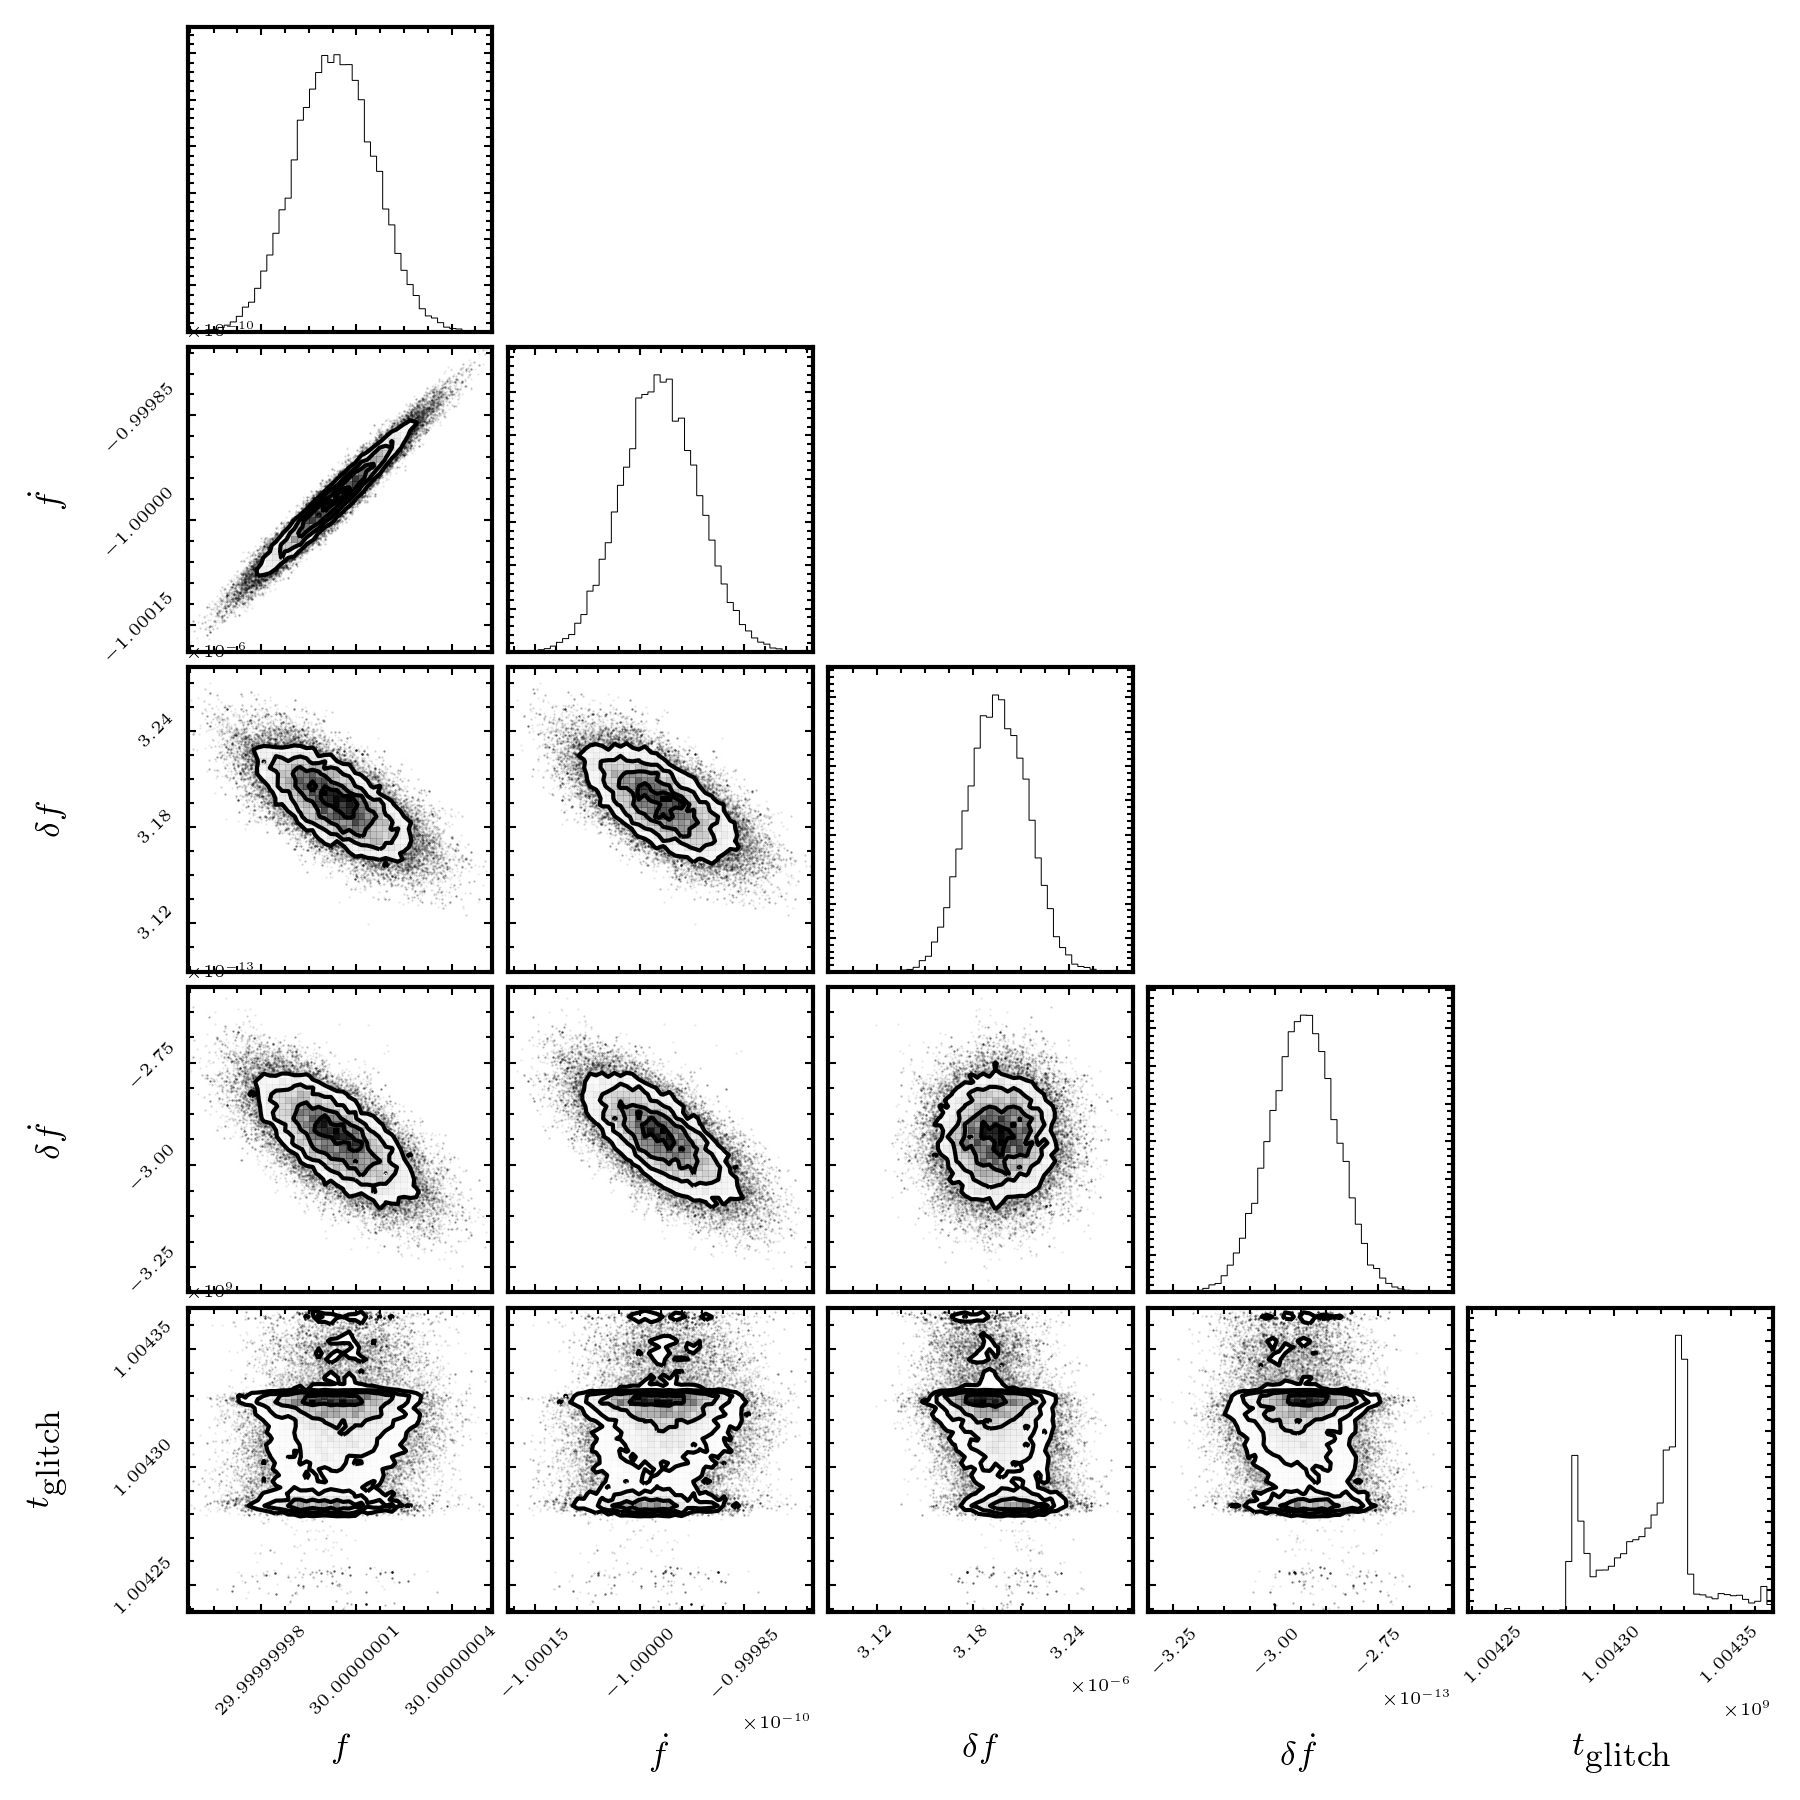
\includegraphics[width=0.5\textwidth]{single_glitch_glitchSearch_corner}
\caption{}
\label{fig_glitch_posteriors}
\end{figure}

\section{Conclusion}
\label{sec_conclusion}



\section{Acknowledgements}

\bibliography{bibliography}

\end{document}
